\section{Notation and analytical preliminaries}\label{sec:B-prelim}

This section collects the calculus, matrix and probability facts that the rest of the appendix uses. Each fact
comes with a short proof or a precise reference. We state the facts in the form in which the chapters apply
them, and we point to those applications as we go.

\subsection{Vectors, derivatives and norms}\label{sec:B-notation}

Vectors are columns unless they are rows of product characteristics, and $^\top$ denotes the transpose. For
$x, y \in \R^n$ we write $x \geq y$ if $x_k \geq y_k$ for every $k$, and $x \gg y$ if every inequality is strict.
The vector of ones is $\mathbf{1}$, the $k$-th unit vector is $e_k$, and the identity matrix is $I_n$, or $I$ when
the size is clear. The indicator function is $\indic\{\cdot\}$. The generic parameter $a$ and the generic choice $x$
follow the conventions stated at the start of the appendix.

Derivatives follow one convention. For a differentiable $f : \R^n \to \R$, the \emph{gradient} $\nabla f(x)$ is
the column vector with entries $\frac{\partial f}{\partial x_k}$. For a differentiable map
$\Psi : \R^n \times \R^m \to \R^n$, written $\Psi(x, a)$, the \emph{Jacobian} $D_x\Psi$ is the $n \times n$ matrix
with $(j, k)$ element $\frac{\partial \Psi_j}{\partial x_k}$. Similarly, $D_a\Psi$ is the $n \times m$ matrix with
$(j, l)$ element $\frac{\partial \Psi_j}{\partial a_l}$. Row $j$ of a Jacobian collects the derivatives of the
$j$-th equation. The \emph{Hessian} $D^2_{xx}f$ has $(k, l)$ element $\frac{\partial^2 f}{\partial x_k\,\partial x_l}$,
and $D^2_{xa}f$ has $(k, l)$ element $\frac{\partial^2 f}{\partial x_k\,\partial a_l}$. A function is $C^r$ if it has
continuous partial derivatives up to order $r$. The Hessian of a $C^2$ function is symmetric by Young's theorem.

The chain rule takes a compact matrix form. Suppose $x(a)$ is differentiable and $h(a) = \Psi(x(a), a)$. Let
$D_a x$ be the $n \times m$ matrix with $(k, l)$ element $\frac{\partial x_k}{\partial a_l}$. Then
\begin{equation}\label{eq:B-chain}
D_a h(a) = D_x\Psi\big(x(a), a\big)\, D_a x(a) + D_a\Psi\big(x(a), a\big).
\end{equation}
Element by element, \eqref{eq:B-chain} reads
$\frac{\partial h_j}{\partial a_l} = \sum_{k} \frac{\partial \Psi_j}{\partial x_k}\frac{\partial x_k}{\partial a_l} + \frac{\partial \Psi_j}{\partial a_l}$.

Two matrices of share derivatives recur in the book. For mean utilities $\delta = (\delta_1, \dots, \delta_J)^\top$, the
matrix $\frac{\partial s}{\partial \delta^\top}$ has $(j, k)$ element $\frac{\partial s_j}{\partial \delta_k}$. For prices,
the matrix $\Delta$ has $(j, k)$ element $\Delta_{jk} = \frac{\partial s_j}{\partial p_k}$. Both follow the Jacobian
convention, so row $j$ describes how product $j$'s share responds to every mean utility or every price.

The orientation of $\Delta$ matters in the multiproduct pricing condition. Firm $f$ owns the products in
$\mathcal{J}_f$ and earns $M\sum_{k \in \mathcal{J}_f}(p_k - mc_k)s_k(p)$, where $M$ is market size. After division
by $M$, the first-order condition for the price of product $j \in \mathcal{J}_f$ is
\begin{equation}\label{eq:B-foc-scalar}
s_j(p) + \sum_{k \in \mathcal{J}_f}(p_k - mc_k)\frac{\partial s_k}{\partial p_j}(p) = 0 .
\end{equation}
The derivative $\frac{\partial s_k}{\partial p_j}$ is the $(k, j)$ element of $\Delta$, which is the $(j, k)$ element of
$\Delta^\top$. Let $\Omega$ be the ownership matrix, with $\Omega_{jk} = 1$ if $j$ and $k$ have the same owner and
$\Omega_{jk} = 0$ otherwise. The \emph{Hadamard} (element-wise) \emph{product} of two matrices of the same size is
$(A \odot B)_{jk} = A_{jk}B_{jk}$. Row $j$ of $(\Omega \odot \Delta^\top)(p - mc)$ is then
\begin{equation*}
\big[(\Omega \odot \Delta^\top)(p - mc)\big]_j = \sum_{k = 1}^{J}\Omega_{jk}\frac{\partial s_k}{\partial p_j}(p_k - mc_k)
= \sum_{k \in \mathcal{J}_f}(p_k - mc_k)\frac{\partial s_k}{\partial p_j} ,
\end{equation*}
because $\Omega_{jk}$ keeps exactly the products of $j$'s owner. Stacking the $J$ conditions \eqref{eq:B-foc-scalar}
gives
\begin{equation}\label{eq:B-foc-matrix}
s(p) + \big(\Omega \odot \Delta(p)^\top\big)(p - mc) = 0 .
\end{equation}
With single-product firms, $\Omega = I$ and row $j$ reads $s_j + (p_j - mc_j)\frac{\partial s_j}{\partial p_j} = 0$.
Solving,
\begin{equation*}
p_j - mc_j = -s_j\Big(\frac{\partial s_j}{\partial p_j}\Big)^{-1} = \Big(-\frac{\partial \ln s_j}{\partial p_j}\Big)^{-1} ,
\end{equation*}
so the dollar markup is the inverse of the own semi-elasticity of demand. \Cref{sec:04-bertrand-matrix} develops
\eqref{eq:B-foc-matrix} in full.

\begin{remark}[Two errors in the matrix condition]\label{rem:B-hadamard}
The ordinary product $\Omega\Delta^\top$ has $(j, k)$ element $\sum_{l}\Omega_{jl}\frac{\partial s_k}{\partial p_l}$. This sum
adds up the effects on $s_k$ of every price that $j$'s owner sets, and it has no economic meaning. The second
error transposes $\Delta$. The matrix $\Omega \odot \Delta$ places $\frac{\partial s_j}{\partial p_k}$, the effect of a
sibling's price on $j$'s share, where the condition needs $\frac{\partial s_k}{\partial p_j}$. When utility is linear in
price, $\Delta$ is symmetric and this error is invisible. That is the case for the logit and for random
coefficients on price, where $\frac{\partial s_j}{\partial p_k} = \int \alpha_i s_{ij}s_{ik}\,\dd F(\nu_i)$ for $k \neq j$
(\cref{prop:08-derivs}). With the utility $\alpha\ln(y_i - p_j)$ of \citet{BerryLevinsohnPakes1995}, the marginal
utility of money $\frac{\alpha}{y_i - p_k}$ depends on the product. Then $\Delta$ is asymmetric, and a transposed
$\Delta$ produces wrong markups.
\end{remark}

Norms measure the size of vectors and matrices. The \emph{sup norm} of $x \in \R^n$ is $\|x\|_\infty = \max_k |x_k|$. A matrix $A$ inherits the \emph{induced norm}
\begin{equation*}
\|A\|_\infty = \sup_{x \neq 0}\frac{\|Ax\|_\infty}{\|x\|_\infty} .
\end{equation*}
By construction $\|Ax\|_\infty \leq \|A\|_\infty\|x\|_\infty$. Applying this twice gives
$\|ABx\|_\infty \leq \|A\|_\infty\|B\|_\infty\|x\|_\infty$, so $\|AB\|_\infty \leq \|A\|_\infty\|B\|_\infty$. We drop the
subscript $\infty$ when no confusion can arise.

\begin{lemma}[Row-sum formula]\label{lem:B-rowsum}
For every real $n \times m$ matrix $A$,
$\|A\|_\infty = \max_{j}\sum_{k}|A_{jk}|$.
\end{lemma}

\begin{proof}
Let $R = \max_j\sum_k|A_{jk}|$. For any $x$ and any row $j$,
\begin{equation*}
|(Ax)_j| = \Big|\sum_k A_{jk}x_k\Big| \leq \sum_k|A_{jk}|\,|x_k| \leq \Big(\sum_k|A_{jk}|\Big)\|x\|_\infty \leq R\,\|x\|_\infty .
\end{equation*}
Taking the maximum over $j$ gives $\|Ax\|_\infty \leq R\|x\|_\infty$, so $\|A\|_\infty \leq R$. For the reverse
inequality, let row $j^*$ attain the maximum. Set $x_k = 1$ if $A_{j^*k} \geq 0$ and $x_k = -1$ otherwise. Then
$\|x\|_\infty = 1$ and $(Ax)_{j^*} = \sum_k|A_{j^*k}| = R$, so $\|A\|_\infty \geq R$.
\end{proof}

The lemma turns a contraction property of a differentiable map into a condition on the row sums of its Jacobian
(\cref{prop:B-jacobian-criterion}). This is why the uniqueness conditions of \citet{Berry1994} and the contraction
conditions of \citet{BerryLevinsohnPakes1995} are both stated as row sums.

\subsection{Concavity, quasi-concavity and homogeneity}\label{sec:B-concavity}

\begin{definition}[Concave and quasi-concave functions]\label{def:B-concave}
Let $X \subseteq \R^n$ be convex and $f : X \to \R$. The function $f$ is \emph{concave} if
$f(\lambda x + (1 - \lambda)y) \geq \lambda f(x) + (1 - \lambda)f(y)$ for all $x, y \in X$ and $\lambda \in [0, 1]$.
It is \emph{strictly concave} if the inequality is strict whenever $x \neq y$ and $\lambda \in (0, 1)$. It is
\emph{convex} if $-f$ is concave. It is \emph{quasi-concave} if
$f(\lambda x + (1 - \lambda)y) \geq \min\{f(x), f(y)\}$, and \emph{strictly quasi-concave} if this inequality is
strict whenever $x \neq y$ and $\lambda \in (0, 1)$.
\end{definition}

Quasi-concavity is equivalent to convexity of every upper contour set $\{x \in X : f(x) \geq u\}$. Every concave
function is quasi-concave, since $\lambda f(x) + (1 - \lambda)f(y) \geq \min\{f(x), f(y)\}$. The converse fails, because
every monotone function of one variable is quasi-concave.

\begin{proposition}[Second-order characterization]\label{prop:B-concave-hessian}
Let $X$ be open and convex and $f \in C^2$ on $X$.
\begin{enumerate}[label=(\alph*)]
  \item The function $f$ is concave if and only if $D^2_{xx}f(x)$ is negative semidefinite at every $x \in X$.
  \item If $D^2_{xx}f(x)$ is negative definite at every $x \in X$, then $f$ is strictly concave.
\end{enumerate}
The converse of (b) fails.
\end{proposition}

\begin{proof}
A function is concave if and only if its restriction to every segment is concave. For $x \in X$ and a direction
$h$, let $g(t) = f(x + th)$ on the interval of $t$ for which $x + th \in X$. The chain rule gives
$g''(t) = h^\top D^2_{xx}f(x + th)\,h$. A $C^2$ function of one variable is concave if and only if $g' $ is
nonincreasing, that is, if and only if $g'' \leq 0$. So $f$ is concave if and only if $h^\top D^2_{xx}f\,h \leq 0$ for all
$x$ and $h$, which is (a). Under the hypothesis of (b), $g'' < 0$ for every $h \neq 0$. Then $g'$ is strictly
decreasing, $g$ is strictly concave, and so is $f$. The function $f(x) = -x^4$ is strictly concave, yet
$f''(0) = 0$.
\end{proof}

\begin{lemma}[First-order bound]\label{lem:B-concave-foc}
Let $f$ be differentiable and concave on an open convex set $X$. Then
$f(y) \leq f(x) + \nabla f(x)^\top(y - x)$ for all $x, y \in X$. In particular, a point $x^*$ with
$\nabla f(x^*) = 0$ maximizes $f$ on $X$.
\end{lemma}

\begin{proof}
For $\lambda \in (0, 1]$, concavity gives $f(x + \lambda(y - x)) \geq f(x) + \lambda[f(y) - f(x)]$. Rearranging,
\begin{equation*}
\frac{f(x + \lambda(y - x)) - f(x)}{\lambda} \geq f(y) - f(x) .
\end{equation*}
As $\lambda \to 0$ the left side converges to the directional derivative $\nabla f(x)^\top(y - x)$.
\end{proof}

\begin{lemma}[Minimum of affine functions]\label{lem:B-minlinear}
Let $Z$ be convex and let $\{\ell_x : x \in X\}$ be any family of affine functions $\ell_x(z) = b_x + c_x^\top z$ on
$Z$. If $g(z) = \inf_{x \in X}\ell_x(z)$ is finite on $Z$, then $g$ is concave. If
$\bar g(z) = \sup_{x \in X}\ell_x(z)$ is finite on $Z$, then $\bar g$ is convex.
\end{lemma}

\begin{proof}
Take $z, z' \in Z$ and $\lambda \in [0, 1]$. For every $x$, affinity and the definition of $g$ give
\begin{equation*}
\ell_x(\lambda z + (1 - \lambda)z') = \lambda\ell_x(z) + (1 - \lambda)\ell_x(z') \geq \lambda g(z) + (1 - \lambda)g(z') .
\end{equation*}
Taking the infimum over $x$ on the left gives $g(\lambda z + (1 - \lambda)z') \geq \lambda g(z) + (1 - \lambda)g(z')$. The
statement for $\bar g$ follows by applying the first one to the family $-\ell_x$.
\end{proof}

The lemma gives curvature properties of value functions without any differentiability. The expenditure function
$e(p, u) = \min_q\{p^\top q : U(q) \geq u\}$ is a minimum of functions that are linear in $p$, so it is concave in $p$
(\cref{sec:B-duality}). The cost function is concave in input prices for the same reason, and the profit function is
convex in prices because it is a maximum of linear functions (\cref{ex:B-hotelling}).

\begin{lemma}[Maximizers of quasi-concave functions]\label{lem:B-qc-argmax}
If $f$ is quasi-concave on a convex set $X$, its set of maximizers on $X$ is convex. If $f$ is strictly
quasi-concave, it has at most one maximizer.
\end{lemma}

\begin{proof}
Let $V^* = \max_{x \in X}f(x)$, and let $x$ and $y$ be maximizers. For $\lambda \in [0, 1]$, quasi-concavity gives
$f(\lambda x + (1 - \lambda)y) \geq \min\{f(x), f(y)\} = V^*$, so $\lambda x + (1 - \lambda)y$ is a maximizer. If $f$ is
strictly quasi-concave and $x \neq y$, the midpoint satisfies $f\big(\frac{1}{2}x + \frac{1}{2}y\big) > V^*$, which is
impossible.
\end{proof}

Best responses of a player with a quasi-concave payoff are therefore convex-valued. This is the property that
Kakutani's fixed-point theorem needs to deliver existence of a pricing equilibrium (\cref{thm:B-kakutani},
\cref{sec:B-logconcave}).

\begin{definition}[Homogeneity]\label{def:B-homogeneous}
A function $f$ defined on a cone $X \subseteq \R^n$ is \emph{homogeneous of degree $r$} if $f(tx) = t^rf(x)$ for
every $x \in X$ and every $t > 0$.
\end{definition}

\begin{proposition}[Euler's theorem]\label{prop:B-euler}
Let $f$ be differentiable and homogeneous of degree $r$ on an open cone. Then
\begin{enumerate}[label=(\alph*)]
  \item $\sum_{k = 1}^{n}x_k\frac{\partial f}{\partial x_k}(x) = r f(x)$ for every $x$, and
  \item every partial derivative $\frac{\partial f}{\partial x_k}$ is homogeneous of degree $r - 1$.
\end{enumerate}
\end{proposition}

\begin{proof}
Fix $x$ and differentiate the identity $f(tx) = t^rf(x)$ with respect to $t$:
\begin{equation*}
\sum_{k}x_k\frac{\partial f}{\partial x_k}(tx) = r t^{r - 1}f(x) .
\end{equation*}
Setting $t = 1$ gives (a). For (b), differentiate the same identity with respect to $x_k$:
\begin{equation*}
t\,\frac{\partial f}{\partial x_k}(tx) = t^r\frac{\partial f}{\partial x_k}(x) .
\end{equation*}
Dividing by $t$ gives $\frac{\partial f}{\partial x_k}(tx) = t^{r - 1}\frac{\partial f}{\partial x_k}(x)$.
\end{proof}

Euler's theorem produces the adding-up identities of demand theory (\cref{sec:B-duality}). The expenditure function
$e(p, u)$ is homogeneous of degree one in $p$, so $\sum_i p_i\frac{\partial e}{\partial p_i} = e$. Hicksian demand
$h(p, u)$ is homogeneous of degree zero in $p$, so $\sum_j p_j\frac{\partial h_i}{\partial p_j} = 0$, which says that the
Slutsky matrix annihilates the price vector. Marshallian demand $q_i(p, I)$ is homogeneous of degree zero in
$(p, I)$, so
\begin{equation*}
\sum_j p_j\frac{\partial q_i}{\partial p_j} + I\,\frac{\partial q_i}{\partial I} = 0 .
\end{equation*}
Dividing by $q_i$ turns this into the statement that price and income elasticities of each good sum to zero.

\begin{corollary}[Translation invariance]\label{cor:B-translation}
Let $f : \R^n \to \R$ be differentiable with $f(x + c\mathbf{1}) = f(x)$ for all $x$ and all $c \in \R$. Then
\begin{equation*}
\sum_{k = 1}^{n}\frac{\partial f}{\partial x_k}(x) = \nabla f(x)^\top\mathbf{1} = 0 .
\end{equation*}
\end{corollary}

\begin{proof}
The function $c \mapsto f(x + c\mathbf{1})$ is constant, so its derivative at $c = 0$ is zero. By the chain rule
that derivative is $\nabla f(x)^\top\mathbf{1}$.
\end{proof}

The corollary is Euler's theorem in disguise. With $y_k = e^{x_k}$, translation invariance of $f$ is homogeneity of
degree zero of $\tilde f(y) = f(\ln y_1, \dots, \ln y_n)$. Euler's theorem then gives
$0 = \sum_k y_k\frac{\partial \tilde f}{\partial y_k} = \sum_k\frac{\partial f}{\partial x_k}$.

\begin{example}[Shares depend only on utility differences]\label{ex:B-translation-shares}
In an additive random utility model, consumer $i$ obtains $\delta_k + \epsilon_{ik}$ from alternative
$k = 0, 1, \dots, J$. Adding the same constant to every $\delta_k$, the outside good's $\delta_0$ included, leaves
every consumer's choice unchanged. Hence $s_j(\delta + c\mathbf{1}) = s_j(\delta)$ for $\delta = (\delta_0, \dots, \delta_J)$,
and \cref{cor:B-translation} gives
\begin{equation}\label{eq:B-translation-shares}
\sum_{k = 0}^{J}\frac{\partial s_j}{\partial \delta_k} = 0 .
\end{equation}
If the outside good is a substitute for $j$, so that $\frac{\partial s_j}{\partial \delta_0} < 0$, then
\begin{equation*}
\sum_{k = 1}^{J}\frac{\partial s_j}{\partial \delta_k} = -\frac{\partial s_j}{\partial \delta_0} > 0 .
\end{equation*}
This is the step on which \citet[p.~261]{Berry1994} builds his uniqueness argument (\cref{ex:B-share-dd}). In the
logit, $\frac{\partial s_j}{\partial \delta_k} = s_j(\indic\{j = k\} - s_k)$ for $k = 0, \dots, J$, and the sum in
\eqref{eq:B-translation-shares} is $s_j\big(1 - \sum_{k = 0}^{J}s_k\big) = 0$.
\end{example}

\subsection{Mean values, integrals and transformations of random variables}\label{sec:B-calculus}

The scalar mean value theorem says that a function differentiable on $(u, u')$ and continuous on $[u, u']$
satisfies $g(u') - g(u) = g'(\tau)(u' - u)$ for some $\tau \in (u, u')$. For vector-valued maps there is no single
intermediate point, and the right tool is an integral.

\begin{proposition}[Integral form of the mean value theorem]\label{prop:B-mvt-integral}
Let $U \subseteq \R^d$ be open, let $\Psi : U \to \R^n$ be $C^1$, and suppose the segment
$[x, x'] = \{x + t(x' - x) : t \in [0, 1]\}$ lies in $U$. Then
\begin{equation}\label{eq:B-mvt-integral}
\Psi(x') - \Psi(x) = \Big[\int_0^1 D\Psi\big(x + t(x' - x)\big)\,\dd t\Big](x' - x) ,
\end{equation}
where the integral of a matrix is taken element by element.
\end{proposition}

\begin{proof}
For each $j$, the function $g_j(t) = \Psi_j(x + t(x' - x))$ is $C^1$ on $[0, 1]$. The chain rule gives
\begin{equation*}
g_j'(t) = \sum_{k}\frac{\partial \Psi_j}{\partial x_k}\big(x + t(x' - x)\big)(x'_k - x_k) .
\end{equation*}
By the fundamental theorem of calculus, $\Psi_j(x') - \Psi_j(x) = g_j(1) - g_j(0) = \int_0^1 g_j'(t)\,\dd t$. Stacking
the $n$ rows gives \eqref{eq:B-mvt-integral}.
\end{proof}

A single intermediate point does not exist in general. The map $\Psi(t) = (\cos t, \sin t)^\top$ satisfies
$\Psi(2\pi) - \Psi(0) = 0$, while its derivative $(-\sin t, \cos t)^\top$ never vanishes.

\begin{corollary}[Mean value inequality]\label{cor:B-mvi}
Under the assumptions of \cref{prop:B-mvt-integral},
\begin{equation*}
\|\Psi(x') - \Psi(x)\|_\infty \leq \sup_{z \in [x, x']}\|D\Psi(z)\|_\infty\;\|x' - x\|_\infty .
\end{equation*}
\end{corollary}

\begin{proof}
Write $z_t = x + t(x' - x)$. Row $j$ of \eqref{eq:B-mvt-integral} gives
\begin{equation*}
|\Psi_j(x') - \Psi_j(x)| \leq \int_0^1\sum_k\Big|\frac{\partial \Psi_j}{\partial x_k}(z_t)\Big|\,|x'_k - x_k|\,\dd t
\leq \int_0^1\sum_k\Big|\frac{\partial \Psi_j}{\partial x_k}(z_t)\Big|\,\dd t\;\|x' - x\|_\infty .
\end{equation*}
By \cref{lem:B-rowsum} the row sum inside the integral is at most $\|D\Psi(z_t)\|_\infty$. Bounding it by the
supremum over the segment and maximizing over $j$ gives the claim.
\end{proof}

\begin{example}[The mean value step in the BLP contraction]\label{ex:B-blp-mvt}
\citet[Appendix I, p.~887]{BerryLevinsohnPakes1995} study a $C^1$ map $f : \R^J \to \R^J$ whose partial derivatives
are nonnegative and whose row sums $\sum_k\frac{\partial f_j}{\partial x_k}$ are below one. Their operator is
$f(\delta) = \delta + \ln s^{obs} - \ln s(\delta)$, equation (6.8) on p.~865. Take two points $x, x'$ in a bounded box
and let $\lambda = \|x - x'\|_\infty$, so that $x' \leq x + \lambda\mathbf{1}$. Suppose $f_j(x') \geq f_j(x)$. Monotonicity
and \eqref{eq:B-mvt-integral} along the direction $\mathbf{1}$ give
\begin{equation*}
f_j(x') - f_j(x) \leq f_j(x + \lambda\mathbf{1}) - f_j(x)
= \int_0^\lambda\Big[\sum_{k = 1}^{J}\frac{\partial f_j}{\partial x_k}(x + z\mathbf{1})\Big]\dd z \leq \kappa\lambda ,
\end{equation*}
where $\kappa < 1$ is the largest row sum over the compact set of points that the segments can reach. The same bound
follows from \cref{cor:B-mvi}, because with nonnegative partials $\|Df\|_\infty$ is the largest row sum. This step makes
the truncated map a contraction. The full theorem and its proof are in \cref{thm:08-contraction}.
\end{example}

\begin{proposition}[Leibniz's rule]\label{prop:B-leibniz}
\begin{enumerate}[label=(\alph*)]
  \item Let $g(x, a)$ and $g_a(x, a) = \frac{\partial g}{\partial a}(x, a)$ be continuous on
  $[x_L, x_U] \times [a_L, a_U]$, and let $l(a)$ and $m(a)$ be differentiable with values in $[x_L, x_U]$. Then
  $\Gamma(a) = \int_{l(a)}^{m(a)}g(x, a)\,\dd x$ satisfies, for $a \in (a_L, a_U)$,
  \begin{equation}\label{eq:B-leibniz}
  \Gamma'(a) = g\big(m(a), a\big)m'(a) - g\big(l(a), a\big)l'(a) + \int_{l(a)}^{m(a)}g_a(x, a)\,\dd x .
  \end{equation}
  \item Let $\mu$ be a measure, such as the distribution $F$ of a taste shock. Suppose $g(\cdot, a)$ is
  $\mu$-integrable for each $a$ in an open interval $N$ and that $g_a(x, a)$ exists there. Suppose also that an
  integrable function $b(x)$ satisfies $|g_a(x, a)| \leq b(x)$ for all $x$ and all $a \in N$. Then for $a \in N$,
  \begin{equation*}
  \frac{\dd}{\dd a}\int g(x, a)\,\dd\mu(x) = \int g_a(x, a)\,\dd\mu(x) .
  \end{equation*}
\end{enumerate}
\end{proposition}

\begin{proof}
We prove (b) first. For $h \neq 0$ small, the scalar mean value theorem gives
$\frac{g(x, a + h) - g(x, a)}{h} = g_a(x, a + \tau_x h)$ for some $\tau_x \in (0, 1)$. This difference quotient is
bounded by $b(x)$, and it converges to $g_a(x, a)$ as $h \to 0$. Dominated convergence lets us pass the limit
through the integral.

For (a), define $G(u, w, a) = \int_w^u g(x, a)\,\dd x$. The fundamental theorem of calculus gives
$\frac{\partial G}{\partial u} = g(u, a)$ and $\frac{\partial G}{\partial w} = -g(w, a)$. Part (b), with $\mu$ the Lebesgue
measure on $[x_L, x_U]$ and $b$ the maximum of $|g_a|$ on the compact rectangle, gives
$\frac{\partial G}{\partial a} = \int_w^u g_a(x, a)\,\dd x$. These partial derivatives are continuous, so $G$ is $C^1$. The
chain rule applied to $\Gamma(a) = G(m(a), l(a), a)$ gives \eqref{eq:B-leibniz}.
\end{proof}

\begin{example}[Share derivatives with random coefficients]\label{ex:B-rc-derivatives}
In the random coefficients logit, consumer $i$ with taste draw $\nu_i$ buys $j$ with probability
$s_{ij}(p, \nu_i) = \frac{\exp(\delta_j + \mu_{ij})}{1 + \sum_{k}\exp(\delta_k + \mu_{ik})}$. Her price coefficient is $\alpha_i$, so
$\frac{\partial(\delta_k + \mu_{ik})}{\partial p_k} = -\alpha_i$. The logit derivative
$\frac{\partial s_{ij}}{\partial(\delta_k + \mu_{ik})} = s_{ij}(\indic\{j = k\} - s_{ik})$ and the chain rule give
\begin{equation*}
\frac{\partial s_{ij}}{\partial p_k} = \alpha_i\, s_{ij}\big(s_{ik} - \indic\{j = k\}\big) .
\end{equation*}
Market shares are $s_j(p) = \int s_{ij}(p, \nu)\,\dd F(\nu)$. Because shares lie in $[0, 1]$, the integrand's derivative
satisfies $|\alpha_i s_{ij}(s_{ik} - \indic\{j = k\})| \leq |\alpha_i|$ at every price vector. If $\E|\alpha_i| < \infty$,
\cref{prop:B-leibniz}(b) applies with $b = |\alpha_i|$ and
\begin{equation}\label{eq:B-rc-derivative}
\frac{\partial s_j}{\partial p_k} = \int \alpha_i\, s_{ij}\big(s_{ik} - \indic\{j = k\}\big)\,\dd F(\nu_i) .
\end{equation}
With $B$ simulation draws the integral becomes an average over draws (\cref{prop:08-derivs}).
\end{example}

A second application has a variable limit of integration. In first-price auctions with $n$ bidders, values drawn
from $F$, and reserve price $r$, the function $\int_r^v F(t)^{n - 1}\,\dd t$ has derivative $F(v)^{n - 1}$ by
\eqref{eq:B-leibniz} with $l' = 0$, $m(v) = v$ and $g_a = 0$. \Cref{ex:B-auction-envelope} uses this step, and
\cref{sec:B-orderstats} uses Leibniz's rule to derive the densities of order statistics.

\begin{lemma}[Tail formula for the mean]\label{lem:B-tail}
If $X \geq 0$ has CDF $F$, then $\E[X] = \int_0^\infty\big(1 - F(x)\big)\,\dd x$, where both sides may be infinite.
\end{lemma}

\begin{proof}
Write $X = \int_0^\infty\indic\{x < X\}\,\dd x$. Take expectations and exchange the order of integration, which
Tonelli's theorem allows because the integrand is nonnegative:
\begin{equation*}
\E[X] = \int_0^\infty\E\big[\indic\{x < X\}\big]\,\dd x = \int_0^\infty\Pr(X > x)\,\dd x = \int_0^\infty\big(1 - F(x)\big)\,\dd x .
\qedhere
\end{equation*}
\end{proof}

The same exchange of integrals is integration by parts,
$\int_u^{u'}\varphi\,\dd\psi = \varphi(u')\psi(u') - \varphi(u)\psi(u) - \int_u^{u'}\psi\,\dd\varphi$, in probabilistic form. Auction
theory uses it to write bids as conditional expectations.

\begin{example}[The first-price bid as a conditional expectation]\label{ex:B-rs-parts}
Let $Y_1$ be the highest of $n - 1$ rival values, drawn independently from $F$, so its CDF is $F^{n - 1}$. For $v > r$,
consider $\E[\max\{Y_1, r\} \mid Y_1 < v]$. The event $Y_1 \leq r$ has probability $F(r)^{n - 1}$ and contributes $r$, so
\begin{equation*}
\E[\max\{Y_1, r\} \mid Y_1 < v] = \frac{rF(r)^{n - 1} + \int_r^v t\,\dd\big[F(t)^{n - 1}\big]}{F(v)^{n - 1}} .
\end{equation*}
Integration by parts with $\varphi(t) = t$ and $\psi(t) = F(t)^{n - 1}$ gives
\begin{equation*}
\int_r^v t\,\dd\big[F(t)^{n - 1}\big] = vF(v)^{n - 1} - rF(r)^{n - 1} - \int_r^vF(t)^{n - 1}\,\dd t .
\end{equation*}
The boundary terms in $r$ cancel, and
\begin{equation}\label{eq:B-rs-bid}
\E[\max\{Y_1, r\} \mid Y_1 < v] = v - \frac{\int_r^v F(t)^{n - 1}\,\dd t}{F(v)^{n - 1}} .
\end{equation}
The right side is the equilibrium bid of the symmetric first-price auction \citep{RileySamuelson1981}, derived in
\cref{ex:B-auction-envelope} and in \cref{sec:14-fpa-envelope}.
\end{example}

\begin{lemma}[Probability integral transform]\label{lem:B-pit}
\begin{enumerate}[label=(\alph*)]
  \item If $X$ has a continuous CDF $F$, then $F(X)$ is uniformly distributed on $[0, 1]$.
  \item For any CDF $F$, define the generalized inverse $F^{-1}(u) = \inf\{x : F(x) \geq u\}$ for $u \in (0, 1)$. If
  $U$ is uniform on $[0, 1]$, then $F^{-1}(U)$ has CDF $F$.
\end{enumerate}
\end{lemma}

\begin{proof}
Right continuity of $F$ implies that $F^{-1}(u) \leq x$ if and only if $u \leq F(x)$. For (b),
$\Pr(F^{-1}(U) \leq x) = \Pr(U \leq F(x)) = F(x)$. For (a), fix $u \in (0, 1)$. The same equivalence shows that
$F(X) \geq u$ if and only if $X \geq F^{-1}(u)$. Continuity of $F$ gives $\Pr(X \geq x) = 1 - F(x)$ and
$F(F^{-1}(u)) = u$. Hence
\begin{equation*}
\Pr\big(F(X) \geq u\big) = \Pr\big(X \geq F^{-1}(u)\big) = 1 - F\big(F^{-1}(u)\big) = 1 - u ,
\end{equation*}
so $\Pr(F(X) < u) = u$ for every $u \in (0, 1)$, which is the uniform distribution.
\end{proof}

Part (b) is how simulation draws are produced. The standard Gumbel CDF $\exp(-e^{-x})$ has inverse
$-\ln(-\ln u)$, so $-\ln(-\ln U)$ is a standard Gumbel draw (\cref{sec:B-ev}). Part (a) maps order statistics of any
continuous distribution into order statistics of uniforms (\cref{sec:B-orderstats}).

\subsection{Matrix facts}\label{sec:B-matrix}

A symmetric matrix $A$ is \emph{negative semidefinite} if $x^\top Ax \leq 0$ for every $x$, and \emph{negative definite}
if $x^\top Ax < 0$ for every $x \neq 0$. Equivalently, all eigenvalues of $A$ are nonpositive in the first case and
negative in the second. Positive
(semi)definiteness is defined with the inequalities reversed. Second-order conditions for maximization and the
negativity of the Slutsky matrix (\cref{sec:B-duality}) are statements of this kind. In practice they are checked
with determinants.

\begin{proposition}[Principal minors]\label{prop:B-minors}
Let $A$ be a symmetric $n \times n$ matrix and let $A_k$ be its leading $k \times k$ submatrix.
\begin{enumerate}[label=(\alph*)]
  \item $A$ is negative definite if and only if $(-1)^k\det A_k > 0$ for $k = 1, \dots, n$.
  \item $A$ is negative semidefinite if and only if $(-1)^k\det A_S \geq 0$ for every principal submatrix $A_S$ of
  order $k$, formed from any $k$ rows and the same $k$ columns, for every $k$.
\end{enumerate}
\end{proposition}

\Citet{SimonBlume1994} prove both parts. For $n = 2$, part (a) says that $\begin{psmallmatrix} a_{11} & a_{12} \\ a_{12} & a_{22}\end{psmallmatrix}$ is
negative definite if and only if $a_{11} < 0$ and $a_{11}a_{22} - a_{12}^2 > 0$. Part (b) needs every principal minor,
including those that are not leading. The matrix $\begin{psmallmatrix} 0 & 0 \\ 0 & 1\end{psmallmatrix}$ has leading minors $0$ and $0$, which
satisfy the weak sign conditions. Yet it is not negative semidefinite, and its principal minor of order one in the
second position equals $1$.

\begin{lemma}[Diagonal dominance]\label{lem:B-dd}
Let $A$ be a real $n \times n$ matrix.
\begin{enumerate}[label=(\alph*)]
  \item (Gershgorin) Every eigenvalue $z$ of $A$, real or complex, satisfies
  $|A_{jj} - z| \leq \sum_{k \neq j}|A_{jk}|$ for at least one row $j$.
  \item (Levy-Desplanques) If $A$ is \emph{strictly diagonally dominant}, that is,
  $|A_{jj}| > \sum_{k \neq j}|A_{jk}|$ for every row $j$, then $A$ is nonsingular.
  \item If $A$ is symmetric, strictly diagonally dominant and has a negative diagonal, then $A$ is negative definite.
\end{enumerate}
\end{lemma}

\begin{proof}
For (a), let $Ax = zx$ with $x \neq 0$, and pick $j$ with $|x_j| = \|x\|_\infty > 0$. Row $j$ of the eigenvalue equation
reads $(A_{jj} - z)x_j = -\sum_{k \neq j}A_{jk}x_k$. Taking absolute values and dividing by $|x_j|$,
\begin{equation*}
|A_{jj} - z| \leq \sum_{k \neq j}|A_{jk}|\,\frac{|x_k|}{|x_j|} \leq \sum_{k \neq j}|A_{jk}| .
\end{equation*}
For (b), $z = 0$ would require $|A_{jj}| \leq \sum_{k \neq j}|A_{jk}|$ for some row, which strict dominance rules
out. So $0$ is not an eigenvalue and $A$ is nonsingular. For (c), the eigenvalues of a symmetric matrix are real.
By (a) each lies within $\sum_{k \neq j}|A_{jk}| < |A_{jj}| = -A_{jj}$ of some $A_{jj} < 0$, so each is negative.
\end{proof}

\begin{example}[The share Jacobian is invertible]\label{ex:B-share-dd}
Assume, with \citet[p.~260]{Berry1994}, that $\frac{\partial s_j}{\partial \delta_j} > 0$ and
$\frac{\partial s_j}{\partial \delta_k} < 0$ for every $k \neq j$, the outside good included. By
\cref{ex:B-translation-shares},
\begin{equation*}
\frac{\partial s_j}{\partial \delta_j} - \sum_{k \geq 1, k \neq j}\Big|\frac{\partial s_j}{\partial \delta_k}\Big|
= \sum_{k = 1}^{J}\frac{\partial s_j}{\partial \delta_k} = -\frac{\partial s_j}{\partial \delta_0} > 0 .
\end{equation*}
So the $J \times J$ matrix $\frac{\partial s}{\partial \delta^\top}$ of inside goods is strictly diagonally dominant at every
$\delta$. By \cref{lem:B-dd} it is nonsingular. This is Berry's condition (A2), and in the logit the margin of
dominance is $s_js_0$. The implicit function theorem then delivers the derivatives of the inverse share function
(\cref{ex:B-inversion-gradient}).
\end{example}

\begin{lemma}[Neumann series]\label{lem:B-neumann}
Let $\|\cdot\|$ be an induced matrix norm and $\|A\| < 1$. Then $I - A$ is nonsingular,
\begin{equation*}
(I - A)^{-1} = \sum_{h = 0}^{\infty}A^h , \qquad\text{and}\qquad \big\|(I - A)^{-1}\big\| \leq \frac{1}{1 - \|A\|} .
\end{equation*}
\end{lemma}

\begin{proof}
Let $S_H = \sum_{h = 0}^{H}A^h$. Submultiplicativity gives $\|A^h\| \leq \|A\|^h$, so for $H' > H$,
\begin{equation*}
\|S_{H'} - S_H\| \leq \sum_{h = H + 1}^{H'}\|A\|^h \leq \frac{\|A\|^{H + 1}}{1 - \|A\|} \to 0 .
\end{equation*}
The partial sums are therefore Cauchy and converge to a matrix $S$. Telescoping gives
$(I - A)S_H = I - A^{H + 1}$, and $A^{H + 1} \to 0$. Taking limits, $(I - A)S = I$, and $S(I - A) = I$ in the same
way. The bound follows from $\|S_H\| \leq \sum_{h \leq H}\|A\|^h \leq \frac{1}{1 - \|A\|}$.
\end{proof}

The lemma is the linear case of the contraction mapping theorem (\cref{thm:B-banach}). The affine map
$\Phi(x) = Ax + b$ contracts with modulus $\|A\|$, and its iterates from $x^{(0)} = 0$ are $x^{(H)} = S_{H - 1}b$. They
converge to the fixed point $(I - A)^{-1}b$. \Cref{prop:B-cs-nash} reads the series as rounds of strategic responses.

\begin{lemma}[Sherman-Morrison formula]\label{lem:B-sm}
Let $B$ be nonsingular and $u, v$ vectors with $1 - v^\top B^{-1}u \neq 0$. Then
\begin{equation}\label{eq:B-sm}
\big(B - uv^\top\big)^{-1} = B^{-1} + \frac{B^{-1}uv^\top B^{-1}}{1 - v^\top B^{-1}u} .
\end{equation}
\end{lemma}

\begin{proof}
Write $\tau = 1 - v^\top B^{-1}u$ and multiply $B - uv^\top$ by the right side of \eqref{eq:B-sm}:
\begin{align*}
\big(B - uv^\top\big)\Big(B^{-1} + \frac{B^{-1}uv^\top B^{-1}}{\tau}\Big)
&= I + \frac{uv^\top B^{-1}}{\tau} - uv^\top B^{-1} - \frac{u\,(v^\top B^{-1}u)\,v^\top B^{-1}}{\tau} \\
&= I + uv^\top B^{-1}\,\frac{1 - \tau - v^\top B^{-1}u}{\tau} = I ,
\end{align*}
because $1 - \tau = v^\top B^{-1}u$. The scalar $v^\top B^{-1}u$ can be moved in front of $v^\top B^{-1}$ because it
is a number.
\end{proof}

\begin{example}[The logit Jacobian, its inverse, and logit markups]\label{ex:B-logit-jacobian}
In the logit, $s_j = \frac{e^{\delta_j}}{\Lambda}$ with $\Lambda = 1 + \sum_{k = 1}^{J}e^{\delta_k}$ and $s_0 = \frac{1}{\Lambda}$. Since
$\frac{\partial \Lambda}{\partial \delta_k} = e^{\delta_k}$, the quotient rule gives
\begin{equation*}
\frac{\partial s_j}{\partial \delta_j} = \frac{e^{\delta_j}\Lambda - e^{\delta_j}e^{\delta_j}}{\Lambda^2} = s_j(1 - s_j) ,
\qquad
\frac{\partial s_j}{\partial \delta_k} = -\frac{e^{\delta_j}e^{\delta_k}}{\Lambda^2} = -s_js_k \quad (k \neq j) .
\end{equation*}
In matrix form, with $s = (s_1, \dots, s_J)^\top$,
\begin{equation}\label{eq:B-logit-jacobian}
\frac{\partial s}{\partial \delta^\top} = \diag(s) - ss^\top .
\end{equation}
This is a diagonal matrix minus a rank-one matrix, so \cref{lem:B-sm} applies with $B = \diag(s)$ and $u = v = s$.
Two facts do the work:
\begin{equation*}
\diag(s)^{-1}s = \mathbf{1} , \qquad s^\top\diag(s)^{-1}s = s^\top\mathbf{1} = \sum_{k = 1}^{J}s_k = 1 - s_0 .
\end{equation*}
The denominator in \eqref{eq:B-sm} is $1 - (1 - s_0) = s_0 > 0$, and the numerator is $\mathbf{1}\mathbf{1}^\top$. Hence
\begin{equation}\label{eq:B-logit-jacobian-inverse}
\big[\diag(s) - ss^\top\big]^{-1} = \diag\Big(\frac{1}{s_1}, \dots, \frac{1}{s_J}\Big) + \frac{1}{s_0}\mathbf{1}\mathbf{1}^\top .
\end{equation}
A direct check confirms \eqref{eq:B-logit-jacobian-inverse}. The logit inversion $\delta_j = \ln s_j - \ln s_0$ with
$s_0 = 1 - \sum_k s_k$ has $\frac{\partial \delta_j}{\partial s_k} = \frac{\indic\{j = k\}}{s_j} + \frac{1}{s_0}$, which is the
$(j, k)$ element of \eqref{eq:B-logit-jacobian-inverse}, as the inverse function theorem requires.

Markups follow in a few lines. With $\delta_j = \tilde\delta_j - \alpha p_j$, the price Jacobian is
$\Delta = -\alpha\big[\diag(s) - ss^\top\big]$, which is symmetric. Write $m = p - mc$, so \eqref{eq:B-foc-matrix} gives
$m = -(\Omega \odot \Delta^\top)^{-1}s$.
\begin{enumerate}[label=(\roman*)]
  \item Single-product firms. With $\Omega = I$, the matrix $\Omega \odot \Delta^\top$ is diagonal with entries
  $-\alpha s_j(1 - s_j)$. Hence $m_j = \frac{s_j}{\alpha s_j(1 - s_j)} = \frac{1}{\alpha(1 - s_j)}$.
  \item One owner of all inside goods. With $\Omega = \mathbf{1}\mathbf{1}^\top$, we have $\Omega \odot \Delta^\top = \Delta$, and
  \eqref{eq:B-logit-jacobian-inverse} gives
  \begin{equation*}
  m = \frac{1}{\alpha}\Big[\diag\Big(\frac{1}{s_1}, \dots, \frac{1}{s_J}\Big) + \frac{1}{s_0}\mathbf{1}\mathbf{1}^\top\Big]s
  = \frac{1}{\alpha}\Big[\mathbf{1} + \frac{1 - s_0}{s_0}\mathbf{1}\Big] = \frac{1}{\alpha s_0}\mathbf{1} .
  \end{equation*}
  Every product carries the same markup $\frac{1}{\alpha s_0}$.
  \item A multiproduct firm. Order products by owner, so that $\Omega$ is block diagonal. Then $\Omega \odot \Delta^\top$ is
  block diagonal with blocks $-\alpha\big[\diag(s_f) - s_fs_f^\top\big]$, where $s_f$ collects the shares of firm $f$.
  \Cref{lem:B-sm} with $v^\top B^{-1}u = \sum_{k \in \mathcal{J}_f}s_k \equiv S_f$ inverts each block as
  $\diag(s_f)^{-1} + \frac{1}{1 - S_f}\mathbf{1}\mathbf{1}^\top$. The same computation as in (ii) gives the common markup
  \begin{equation*}
  m_k = \frac{1}{\alpha}\Big[1 + \frac{S_f}{1 - S_f}\Big] = \frac{1}{\alpha(1 - S_f)} \qquad\text{for every } k \in \mathcal{J}_f .
  \end{equation*}
\end{enumerate}
Case (iii) contains (i) with $S_f = s_j$ and (ii) with $S_f = 1 - s_0$. \Cref{prop:04-logit-markup} derives the same
formula from the scalar conditions, and \cref{sec:B-logit-algebra} reuses the example.
\end{example}

\section{The implicit function theorem and comparative statics}\label{sec:B-ift}

Equilibrium conditions rarely solve for the endogenous variables in closed form. First-order conditions,
market-clearing conditions and share equations define prices, quantities or mean utilities only implicitly, as
solutions $x$ of a system $\Psi(x, a) = 0$. Yet we need to know how the solution moves with costs, taxes, ownership
or demand parameters. The implicit function theorem says when the solution is a differentiable function $x(a)$,
and it gives the derivative without solving the system.

\subsection{Statement and proof}\label{sec:B-ift-statement}

\begin{theorem}[Implicit function theorem, scalar case]\label{thm:B-ift-scalar}
Let $\Psi : \R \times \R^m \to \R$ be $C^1$ near $(x_0, a_0)$, with $\Psi(x_0, a_0) = 0$ and $\Psi_x(x_0, a_0) \neq 0$.
Then there are open neighborhoods $N_a$ of $a_0$ and $N_x$ of $x_0$, and a unique function $x : N_a \to N_x$, such that
$\Psi(x(a), a) = 0$ for every $a \in N_a$. The function $x(\cdot)$ is $C^1$, and
\begin{equation}\label{eq:B-ift-scalar}
\frac{\partial x}{\partial a_l}(a) = -\frac{\Psi_{a_l}\big(x(a), a\big)}{\Psi_x\big(x(a), a\big)} , \qquad l = 1, \dots, m .
\end{equation}
\end{theorem}

\begin{proof}
We proceed in five steps.
\begin{enumerate}[label=Step \arabic*., leftmargin=*, align=left]
  \item Replacing $\Psi$ by $-\Psi$ if necessary, assume $\Psi_x(x_0, a_0) > 0$. By continuity of $\Psi_x$ there are
  $\epsilon > 0$ and $\eta > 0$ with $\Psi_x(x, a) > 0$ whenever $|x - x_0| \leq \epsilon$ and $\|a - a_0\| \leq \eta$. For
  each such $a$, the function $\Psi(\cdot, a)$ is strictly increasing on $[x_0 - \epsilon, x_0 + \epsilon]$.
  \item Since $\Psi(x_0, a_0) = 0$ and $\Psi(\cdot, a_0)$ is strictly increasing,
  $\Psi(x_0 - \epsilon, a_0) < 0 < \Psi(x_0 + \epsilon, a_0)$. By continuity of $\Psi$ in $a$, there is $\eta' \in (0, \eta]$
  such that $\Psi(x_0 - \epsilon, a) < 0 < \Psi(x_0 + \epsilon, a)$ for all $\|a - a_0\| < \eta'$.
  \item Let $N_a = \{a : \|a - a_0\| < \eta'\}$ and $N_x = (x_0 - \epsilon, x_0 + \epsilon)$. For $a \in N_a$, the intermediate
  value theorem gives a root $x(a) \in N_x$. Strict monotonicity makes it the only root in $N_x$.
  \item The function $x(\cdot)$ is continuous. At any $a_1 \in N_a$, repeat Steps 1 to 3 around $(x(a_1), a_1)$ with an
  arbitrary $\epsilon' > 0$ in place of $\epsilon$. For $a$ close enough to $a_1$, the unique root then lies within
  $\epsilon'$ of $x(a_1)$.
  \item Fix $a \in N_a$ and $l$, let $a' = a + h e_l$, and write $\Delta x = x(a') - x(a)$. Apply the scalar mean value
  theorem to $\tau \mapsto \Psi(x(a) + \tau\Delta x, a + \tau h e_l)$ on $[0, 1]$. Since $\Psi$ vanishes at both ends,
  \begin{equation*}
  0 = \Psi(x(a'), a') - \Psi(x(a), a) = \Psi_x(\xi)\,\Delta x + \Psi_{a_l}(\xi)\,h
  \end{equation*}
  for a point $\xi$ on the segment between $(x(a), a)$ and $(x(a'), a')$. Hence
  $\frac{\Delta x}{h} = -\frac{\Psi_{a_l}(\xi)}{\Psi_x(\xi)}$. As $h \to 0$, Step 4 gives $\Delta x \to 0$, so
  $\xi \to (x(a), a)$. Continuity of the partial derivatives yields \eqref{eq:B-ift-scalar}. The right side of
  \eqref{eq:B-ift-scalar} is continuous in $a$, so $x(\cdot)$ is $C^1$. \qedhere
\end{enumerate}
\end{proof}

\Cref{fig:B-ift} illustrates the theorem with $\Psi(x, a) = x^2 + a^2 - 1$, whose zero set is the unit circle. Here
$\Psi_x = 2x$ and $\Psi_a = 2a$. At $(a_0, x_0) = (0.6, 0.8)$ we have $\Psi_x = 1.6 \neq 0$. The theorem gives the
local solution $x(a) = \sqrt{1 - a^2}$ with slope
\begin{equation*}
x'(a_0) = -\frac{\Psi_a}{\Psi_x} = -\frac{2a_0}{2x_0} = -\frac{3}{4} ,
\end{equation*}
which matches the direct derivative $-\frac{a_0}{\sqrt{1 - a_0^2}}$. At $(1, 0)$, by contrast, $\Psi_x = 0$. In every box
around that point there are two solutions $\pm\sqrt{1 - a^2}$ for $a$ slightly below one and none for $a > 1$.

\begin{figure}[htbp]
\centering
\begin{tikzpicture}[x=2.3cm, y=2.3cm, >=Stealth]
  \draw[->] (-1.3,0) -- (1.55,0) node[right] {$a$};
  \draw[->] (0,-1.25) -- (0,1.35) node[above] {$x$};
  \draw[thick, black!45] (0,0) circle (1);
  \node[black!70, font=\small] at (-0.95,0.9) {$x^2 + a^2 = 1$};
  \draw[dashed, blue!60!black] (0.38,0.52) rectangle (0.84,1.04);
  \draw[very thick, blue!60!black, domain=0.38:0.84, samples=40, variable=\t] plot ({\t},{sqrt(1-\t*\t)});
  \draw[red!70!black, thick] (0.2,1.1) -- (1.05,0.4625);
  \fill[blue!60!black] (0.6,0.8) circle (0.022);
  \draw[->, black!70] (1.12,0.98) -- (0.64,0.82);
  \node[anchor=west, font=\small, align=left] at (1.12,1.02) {regular point $(a_0, x_0) = (0.6, 0.8)$,\\ unique local solution $x(a)$};
  \draw[->, black!70] (1.12,0.62) -- (0.93,0.56);
  \node[anchor=west, font=\small] at (1.12,0.62) {tangent with slope $-\frac{a_0}{x_0} = -\frac{3}{4}$};
  \draw[dashed, orange!80!black] (0.8,-0.36) rectangle (1.22,0.36);
  \draw[very thick, orange!80!black, domain=0.9367:1, samples=30, variable=\t] plot ({\t},{sqrt(1-\t*\t)});
  \draw[very thick, orange!80!black, domain=0.9367:1, samples=30, variable=\t] plot ({\t},{-sqrt(1-\t*\t)});
  \fill[orange!80!black] (1,0) circle (0.022);
  \draw[->, black!70] (1.3,-0.3) -- (1.03,-0.03);
  \node[anchor=west, font=\small, align=left] at (1.3,-0.38) {fold point $(1, 0)$, where $\Psi_x = 2x = 0$,\\ two solutions for $a < 1$, none for $a > 1$};
\end{tikzpicture}
\caption{The implicit function theorem for $\Psi(x, a) = x^2 + a^2 - 1$. Near the regular point $(0.6, 0.8)$ the zero set is
the graph of a unique $C^1$ function, whose slope $-\frac{\Psi_a}{\Psi_x} = -\frac{3}{4}$ is the slope of the tangent. Near the fold
point $(1, 0)$, where $\Psi_x = 0$, no box contains the graph of a unique function of $a$.}
\label{fig:B-ift}
\end{figure}

\begin{theorem}[Implicit function theorem]\label{thm:B-ift}
Let $\Psi : U \to \R^n$ be $C^1$ on an open set $U \subseteq \R^n \times \R^m$. Let $(x_0, a_0) \in U$ satisfy
$\Psi(x_0, a_0) = 0$, with $D_x\Psi(x_0, a_0)$ nonsingular. Then there are $\epsilon > 0$ and $\eta > 0$ with the following
property. For every $a$ with $\|a - a_0\| < \eta$, the system $\Psi(x, a) = 0$ has exactly one solution $x(a)$ with
$\|x(a) - x_0\| \leq \epsilon$. The function $x(\cdot)$ is $C^1$, and
\begin{equation}\label{eq:B-ift}
D_a x(a) = -\big[D_x\Psi\big(x(a), a\big)\big]^{-1}D_a\Psi\big(x(a), a\big) .
\end{equation}
\end{theorem}

\begin{proof}
All norms are sup norms and their induced matrix norms. We first derive \eqref{eq:B-ift} assuming that a
differentiable solution exists, and then prove existence, uniqueness and differentiability.

\emph{The derivative formula.} The function $h(a) = \Psi(x(a), a)$ is identically zero, so its Jacobian is zero. By
the chain rule \eqref{eq:B-chain},
\begin{align*}
0 &= D_a h(a) \\
  &= D_x\Psi\big(x(a), a\big)\,D_a x(a) + D_a\Psi\big(x(a), a\big) .
\end{align*}
Moving the second term to the left and premultiplying by $[D_x\Psi]^{-1}$ gives \eqref{eq:B-ift}.

\emph{Existence and uniqueness.} Let $J_0 = D_x\Psi(x_0, a_0)$ and define
\begin{equation*}
\Phi_a(x) = x - J_0^{-1}\Psi(x, a) .
\end{equation*}
Since $J_0^{-1}$ is nonsingular, $x$ is a fixed point of $\Phi_a$ exactly when $\Psi(x, a) = 0$. The Jacobian of $\Phi_a$ is
\begin{equation*}
D\Phi_a(x) = I - J_0^{-1}D_x\Psi(x, a) = J_0^{-1}\big[J_0 - D_x\Psi(x, a)\big] ,
\end{equation*}
which vanishes at $(x_0, a_0)$. By continuity of $D_x\Psi$, choose $\epsilon > 0$ and $\eta_1 > 0$ such that
$\|D\Phi_a(x)\| \leq \frac{1}{2}$ whenever $\|x - x_0\| \leq \epsilon$ and $\|a - a_0\| \leq \eta_1$. On the closed ball
$B_\epsilon = \{x : \|x - x_0\| \leq \epsilon\}$, which is convex, \cref{cor:B-mvi} gives
\begin{equation}\label{eq:B-ift-contraction}
\|\Phi_a(x) - \Phi_a(x')\| \leq \frac{1}{2}\|x - x'\| \qquad\text{for all } x, x' \in B_\epsilon .
\end{equation}
The map also sends $B_\epsilon$ into itself for $a$ close to $a_0$. For $x \in B_\epsilon$,
\begin{equation*}
\|\Phi_a(x) - x_0\| \leq \|\Phi_a(x) - \Phi_a(x_0)\| + \|\Phi_a(x_0) - x_0\| \leq \frac{\epsilon}{2} + \big\|J_0^{-1}\Psi(x_0, a)\big\| .
\end{equation*}
The last term is zero at $a = a_0$ and continuous in $a$. So there is $\eta \in (0, \eta_1]$ with
$\|J_0^{-1}\Psi(x_0, a)\| \leq \frac{\epsilon}{2}$ for $\|a - a_0\| < \eta$. For such $a$, $\Phi_a$ maps the complete set
$B_\epsilon$ into itself and contracts with modulus $\frac{1}{2}$. The contraction mapping theorem (\cref{thm:B-banach}) gives a
unique fixed point $x(a) \in B_\epsilon$.

\emph{Continuity.} For two parameter values $a, a'$, add and subtract $\Phi_a(x(a'))$ and use
\eqref{eq:B-ift-contraction}:
\begin{equation*}
\|x(a) - x(a')\| \leq \frac{1}{2}\|x(a) - x(a')\| + \big\|J_0^{-1}\big[\Psi(x(a'), a) - \Psi(x(a'), a')\big]\big\| .
\end{equation*}
Hence $\|x(a) - x(a')\| \leq 2\|J_0^{-1}\|\,\sup_{y \in B_\epsilon}\|\Psi(y, a) - \Psi(y, a')\|$. The supremum vanishes as $a' \to a$,
because $\Psi$ is uniformly continuous on compact sets.

\emph{Differentiability.} Fix $a$, write $x = x(a)$ and $x' = x(a')$, and let $z_t$ be the point
$(x + t(x' - x), a + t(a' - a))$. \Cref{prop:B-mvt-integral}, applied to $\Psi$ as a function of the stacked vector
$(x, a)$, gives
\begin{equation*}
0 = \Psi(x', a') - \Psi(x, a) = M_x\,(x' - x) + M_a\,(a' - a) ,
\end{equation*}
where $M_x = \int_0^1 D_x\Psi(z_t)\,\dd t$ and $M_a = \int_0^1 D_a\Psi(z_t)\,\dd t$.
The points $z_t$ stay in the region where $\|I - J_0^{-1}D_x\Psi\| \leq \frac{1}{2}$, so
$\|I - J_0^{-1}M_x\| \leq \frac{1}{2}$. \Cref{lem:B-neumann} makes $J_0^{-1}M_x$, and hence $M_x$, nonsingular. Therefore
$x' - x = -M_x^{-1}M_a(a' - a)$. As $a' \to a$, continuity gives $x' \to x$, $M_x \to D_x\Psi(x, a)$ and
$M_a \to D_a\Psi(x, a)$. So $x(\cdot)$ is differentiable with derivative \eqref{eq:B-ift}, which is continuous in $a$.
\end{proof}

\begin{remark}[The theorem is local]\label{rem:B-ift-local}
The theorem guarantees a unique solution only near $(x_0, a_0)$. It says nothing about solutions far from $x_0$.
Several price equilibria, for instance, can each be locally unique, with a nonsingular Jacobian at each one. Global
uniqueness needs other tools, such as contractions or dominant-diagonal conditions (\cref{sec:B-fixedpoint}). The
theorem also fails where $D_x\Psi$ is singular. At such fold points a small change in $a$ can make solutions
appear, disappear or jump, as at $(1, 0)$ in \cref{fig:B-ift}.
\end{remark}

\subsection{Comparative statics of optima and equilibria}\label{sec:B-cs-optimum}

\begin{proposition}[Comparative statics of an optimum]\label{prop:B-cs-optimum}
Let $f(x, a)$ be $C^2$ with $x$ in an open set $X \subseteq \R^n$. Suppose $x_0$ is an interior maximizer at $a_0$ with
$\nabla_x f(x_0, a_0) = 0$ and $D^2_{xx}f(x_0, a_0)$ negative definite. Then near $a_0$ there is a $C^1$ function
$x^*(a)$ of strict local maximizers with $x^*(a_0) = x_0$, and
\begin{equation}\label{eq:B-cs-optimum}
D_a x^*(a) = -\big[D^2_{xx}f(x^*(a), a)\big]^{-1}D^2_{xa}f(x^*(a), a) .
\end{equation}
In the scalar case $\frac{\dd x^*}{\dd a} = -\frac{f_{xa}}{f_{xx}}$, which has the sign of the cross partial $f_{xa}$.
\end{proposition}

\begin{proof}
Apply \cref{thm:B-ift} to $\Psi(x, a) = \nabla_x f(x, a)$. Its Jacobian $D_x\Psi = D^2_{xx}f$ is negative definite, hence
nonsingular, and $D_a\Psi = D^2_{xa}f$. This gives a $C^1$ solution of the first-order conditions and the formula
\eqref{eq:B-cs-optimum}. The leading principal minors of the Hessian are continuous, so by \cref{prop:B-minors} the
Hessian stays negative definite near $(x_0, a_0)$. The second-order sufficient condition therefore holds along the
solution. In the scalar case $f_{xx} < 0$, so $-\frac{f_{xa}}{f_{xx}}$ has the sign of $f_{xa}$.
\end{proof}

The cross partial $f_{xa}$ measures complementarity between the choice and the parameter. When $f_{xa} > 0$, a
higher $a$ raises the marginal return to $x$, and the optimal $x$ rises. \Cref{sec:B-supermod} obtains the same
monotonicity without differentiability or concavity, by Topkis's theorem.

\begin{example}[Monopoly price and cost]\label{ex:B-monopoly-cs}
A monopolist with constant marginal cost $c$ chooses $p$ to maximize $f(p, c) = (p - c)Q(p)$. The derivatives are
\begin{equation*}
f_p = Q + (p - c)Q' , \qquad f_{pp} = 2Q' + (p - c)Q'' , \qquad f_{pc} = -Q' > 0 .
\end{equation*}
So the price rises with cost whenever the second-order condition $f_{pp} < 0$ holds. The magnitude is
$\frac{\dd p^*}{\dd c} = -\frac{f_{pc}}{f_{pp}} = \frac{Q'}{2Q' + (p - c)Q''}$, the monopoly pass-through rate that
\cref{sec:B-passthrough} studies in detail.
\end{example}

Games add strategic feedback. Each player's first-order condition depends on the others' choices, so a parameter
change moves every player's best response and then moves it again through the rivals' reactions.

\begin{proposition}[Comparative statics of a Nash equilibrium]\label{prop:B-cs-nash}
Players $i = 1, \dots, N$ choose $x_i$ in open intervals, with $C^2$ payoffs $\pi_i(x, a)$ and a scalar parameter $a$.
Let $x^*$ be an interior Nash equilibrium at $a_0$, so that $\Psi_i(x, a) \equiv \frac{\partial \pi_i}{\partial x_i}(x, a) = 0$
for every $i$. Let $D_x\Psi$ be the $N \times N$ matrix with $(i, j)$ element $\frac{\partial^2 \pi_i}{\partial x_i\,\partial x_j}$.
\begin{enumerate}[label=(\alph*)]
  \item If $D_x\Psi(x^*, a_0)$ is nonsingular, the equilibrium is locally a $C^1$ function of $a$ with
  $\frac{\dd x^*}{\dd a} = -[D_x\Psi]^{-1}D_a\Psi$.
  \item Suppose also that $\frac{\partial^2 \pi_i}{\partial x_i^2} < 0$ for every $i$. Define the best-response slopes and the
  direct effects
  \begin{equation*}
  R_{ij} = -\Big(\frac{\partial^2 \pi_i}{\partial x_i^2}\Big)^{-1}\frac{\partial^2 \pi_i}{\partial x_i\,\partial x_j}\ \ (j \neq i),
  \qquad R_{ii} = 0 ,
  \qquad c_i = -\Big(\frac{\partial^2 \pi_i}{\partial x_i^2}\Big)^{-1}\frac{\partial^2 \pi_i}{\partial x_i\,\partial a} .
  \end{equation*}
  Then $\frac{\dd x^*}{\dd a} = (I - R)^{-1}c$. If $\|R\|_\infty < 1$, then
  $\frac{\dd x^*}{\dd a} = \sum_{h = 0}^{\infty}R^hc$.
\end{enumerate}
\end{proposition}

\begin{proof}
Part (a) is \cref{thm:B-ift}. For (b), write $\pi_{ij}$ for $\frac{\partial^2 \pi_i}{\partial x_i\,\partial x_j}$ and
$\pi_{ia}$ for $\frac{\partial^2 \pi_i}{\partial x_i\,\partial a}$. Row $i$ of $D_x\Psi\frac{\dd x^*}{\dd a} + D_a\Psi = 0$ reads
\begin{equation*}
\pi_{ii}\frac{\dd x_i^*}{\dd a} + \sum_{j \neq i}\pi_{ij}\frac{\dd x_j^*}{\dd a} + \pi_{ia} = 0 .
\end{equation*}
Dividing by $-\pi_{ii} > 0$ and rearranging,
\begin{equation*}
\frac{\dd x_i^*}{\dd a} = \sum_{j \neq i}R_{ij}\frac{\dd x_j^*}{\dd a} + c_i .
\end{equation*}
Stacking gives $(I - R)\frac{\dd x^*}{\dd a} = c$. Since $I - R = \diag(\pi_{11}, \dots, \pi_{NN})^{-1}D_x\Psi$, the matrix
$I - R$ is nonsingular, and the series form follows from \cref{lem:B-neumann}.
\end{proof}

The objects in (b) have direct interpretations. Apply \cref{thm:B-ift-scalar} to player $i$'s own first-order
condition. Then $R_{ij}$ is the slope of $i$'s best response to $x_j$. Likewise, $c_i$ is the shift of that best
response when $a$ moves with rivals held fixed. The series says that the equilibrium response is the direct effect $c$, plus the
rivals' reactions $Rc$ to it, plus the reactions $R^2c$ to those reactions, and so on.

\begin{remark}[Stability and the correspondence principle]\label{rem:B-correspondence}
The condition $\|R\|_\infty < 1$ has a dynamic reading. Near $x^*$, best-response dynamics
$x^{(h + 1)} = BR(x^{(h)})$ are approximately $x^{(h + 1)} - x^* = R(x^{(h)} - x^*)$. If every absolute row sum of $R$ is
below one, deviations shrink and the equilibrium is locally stable. With strategic complements
(\cref{def:B-strategic}), $R \geq 0$, so
$(I - R)^{-1} = \sum_h R^h \geq 0$ element by element. A shock that raises every direct effect then raises every
equilibrium action. Stability thus delivers sign restrictions on comparative statics. This is the correspondence
principle of \citet{Samuelson1947}, which \citet{Dixit1986} applies to oligopoly. With strategic substitutes, as in
Cournot, the terms of the series alternate in sign, and stability alone signs fewer responses.
\end{remark}

\subsection{Application: pass-through}\label{sec:B-passthrough}

The \emph{pass-through} rate $\rho = \frac{\dd p}{\dd c}$ is the response of an equilibrium price to a shift in
marginal cost, or $\frac{\dd p}{\dd t}$ for a specific tax $t$. It governs tax incidence, the price effects of
mergers, and tests of market power (\cref{sec:02-passthrough}, \cref{ch:conduct}, \cref{ch:mergers}). Every formula
below comes from one recipe. We write the equilibrium condition as $\Psi(\text{price or quantity}, \text{cost}) = 0$
and apply the implicit function theorem.

The formulas depend on the curvature of demand. As in \eqref{eq:02-chi}, the \emph{curvature} of inverse demand
$P(q)$ is
\begin{equation}\label{eq:B-chi}
\chi(q) = -\frac{qP''(q)}{P'(q)} .
\end{equation}
Since $P' < 0$, $\chi$ has the sign of $P''$. Linear inverse demand has $\chi = 0$, concave inverse demand has
$\chi \leq 0$, and convex inverse demand has $\chi \geq 0$.

\begin{proposition}[Monopoly pass-through]\label{prop:B-passthrough-monopoly}
A monopolist has constant marginal cost $c$ and faces a $C^2$ demand $Q(p)$ with $Q' < 0$. Its optimal price $p(c)$ is
interior and satisfies the first-order condition $Q'(p)(p - c) + Q(p) = 0$ and the strict second-order condition
$(p - c)Q''(p) + 2Q'(p) < 0$. Let $P = Q^{-1}$ be inverse demand and $q = Q(p)$. Then
\begin{equation}\label{eq:B-pt-monopoly}
\rho = \frac{\dd p}{\dd c} = \frac{Q'}{(p - c)Q'' + 2Q'} = \frac{1}{2 - \frac{QQ''}{(Q')^2}} = \frac{1}{2 - \chi(q)} > 0 ,
\end{equation}
and in particular $\frac{QQ''}{(Q')^2} = \chi(q)$.
\end{proposition}

\begin{proof}
Let $\Psi(p, c) = Q'(p)(p - c) + Q(p)$. Its partial derivatives are
\begin{align*}
\Psi_p &= Q''(p)(p - c) + Q'(p) + Q'(p) = (p - c)Q'' + 2Q' , \\
\Psi_c &= -Q'(p) .
\end{align*}
The second-order condition gives $\Psi_p < 0$, so \cref{thm:B-ift-scalar} applies:
\begin{equation*}
\rho = -\frac{\Psi_c}{\Psi_p} = \frac{Q'}{(p - c)Q'' + 2Q'} .
\end{equation*}
Both numerator and denominator are negative, so $\rho > 0$. The same result follows from differentiating the identity
$Q'(p(c))(p(c) - c) + Q(p(c)) \equiv 0$ term by term, which gives $\rho(p - c)Q'' + (\rho - 1)Q' + \rho Q' = 0$.

For the second form, the first-order condition gives $p - c = -\frac{Q}{Q'}$. Substituting,
\begin{equation*}
\rho = \frac{Q'}{-\frac{QQ''}{Q'} + 2Q'} .
\end{equation*}
Dividing numerator and denominator by $Q'$ gives $\rho = \big[2 - \frac{QQ''}{(Q')^2}\big]^{-1}$.

For the third form, differentiate the identity $Q(P(q)) = q$ twice:
\begin{align*}
Q'(P(q))\,P'(q) &= 1 , \\
Q''(P(q))\,P'(q)^2 + Q'(P(q))\,P''(q) &= 0 .
\end{align*}
The first line gives $Q' = \frac{1}{P'}$. The second then gives $Q'' = -\frac{Q'P''}{(P')^2} = -\frac{P''}{(P')^3}$. Hence
\begin{equation*}
\frac{QQ''}{(Q')^2} = q\cdot\Big(-\frac{P''}{(P')^3}\Big)\cdot(P')^2 = -\frac{qP''}{P'} = \chi(q) .
\end{equation*}
The quantity-space route gives the same answer. The condition $P(q) + qP'(q) = c$ has derivative
$2P' + qP''$ in $q$, so $\frac{\dd q}{\dd c} = \frac{1}{2P' + qP''}$ and
$\rho = P'\frac{\dd q}{\dd c} = \frac{P'}{2P' + qP''} = \frac{1}{2 - \chi}$.
\end{proof}

\begin{corollary}[Pass-through and log-concavity]\label{cor:B-passthrough-logconcave}
Under the assumptions of \cref{prop:B-passthrough-monopoly}, monopoly pass-through is below one if and only if
demand is strictly log-concave at $p$, that is, $(\ln Q)''(p) < 0$. It equals one if and only if $(\ln Q)''(p) = 0$,
and it exceeds one if and only if $(\ln Q)''(p) > 0$ \citep{BulowPfleiderer1983}.
\end{corollary}

\begin{proof}
Differentiating $\ln Q$ twice,
\begin{equation*}
(\ln Q)'' = \Big(\frac{Q'}{Q}\Big)' = \frac{QQ'' - (Q')^2}{Q^2} = \frac{(Q')^2}{Q^2}\big(\chi - 1\big) ,
\end{equation*}
by \cref{prop:B-passthrough-monopoly}. The second-order condition makes $2 - \chi > 0$. So $\rho < 1$ if and only if
$2 - \chi > 1$, that is $\chi < 1$, which is $(\ln Q)'' < 0$. The other two cases are identical with the
inequalities replaced.
\end{proof}

The same corollary appears in \cref{cor:02-bulow-pfleiderer}. With unit demand, $Q(p) = M[1 - F(p)]$ for a CDF $F$
of valuations, so demand is log-concave exactly when the survival function $1 - F$ is. \Cref{prop:B-lc-monopoly}
develops this reading and extends the corollary from a local to a global statement.

\begin{example}[Pass-through for common demand curves]\label{ex:B-passthrough}
Each case applies \eqref{eq:B-pt-monopoly}, and \cref{tab:02-pt-examples} collects the results. The symbols
$a$, $b$, $A$ and $\gamma$ follow \cref{ch:theory} and are local to this example and to \cref{prop:B-constant-pt}.
\begin{enumerate}[label=(\roman*)]
  \item \emph{Power inverse demand}, $P(q) = a - bq^{\gamma}$ with $b\gamma > 0$ and $\gamma > -1$. Then
  $P' = -b\gamma q^{\gamma - 1}$ and $P'' = -b\gamma(\gamma - 1)q^{\gamma - 2}$, so $\frac{qP''}{P'} = \gamma - 1$ and
  $\chi = 1 - \gamma$. Directly, marginal revenue is $a - b(1 + \gamma)q^{\gamma}$. Substituting $bq^{\gamma} = a - p$
  gives marginal revenue $(1 + \gamma)p - \gamma a$. Setting it equal to $c$,
  \begin{equation*}
  p = \frac{c + \gamma a}{1 + \gamma} , \qquad \rho = \frac{1}{1 + \gamma} = \frac{1}{2 - \chi} .
  \end{equation*}
  Linear demand is $\gamma = 1$, with $\rho = \frac{1}{2}$.
  \item \emph{Exponential demand}, $P(q) = a - b\ln q$ with $b > 0$, or $Q(p) = e^{\frac{a - p}{b}}$, whose
  semi-elasticity is the constant $\frac{1}{b}$. Then $P' = -\frac{b}{q}$, $P'' = \frac{b}{q^2}$ and $\chi = 1$. Marginal
  revenue is $P + qP' = p - b$, so $p = c + b$ and $\rho = 1$. A monopolist facing this demand passes through
  exactly the cost change, as a competitive industry with flat marginal cost would. A pass-through test cannot tell
  the two apart.
  \item \emph{Constant elasticity}, $Q(p) = Ap^{-\varepsilon}$ with $\varepsilon > 1$, so $P(q) = (\frac{q}{A})^{-\frac{1}{\varepsilon}}$.
  Then $P' = -\frac{P}{\varepsilon q}$ and $P'' = \frac{1}{\varepsilon}(1 + \frac{1}{\varepsilon})\frac{P}{q^2}$, so
  $\chi = 1 + \frac{1}{\varepsilon}$ and
  \begin{equation*}
  \rho = \frac{1}{1 - \frac{1}{\varepsilon}} = \frac{\varepsilon}{\varepsilon - 1} > 1 .
  \end{equation*}
  This matches the pricing rule $p = \frac{\varepsilon}{\varepsilon - 1}c$. In the notation of case (i) it is the power
  family with a zero intercept, $b = -A^{\frac{1}{\varepsilon}}$ and $\gamma = -\frac{1}{\varepsilon}$.
  \item \emph{Logit, one product, rivals' prices fixed}. The share is $s(p) = \frac{e^{\xi - \alpha p}}{\Lambda_{-j} + e^{\xi - \alpha p}}$,
  where $\Lambda_{-j} = 1 + \sum_{k \neq j}e^{\delta_k}$ does not depend on $p$. Then $s' = -\alpha s(1 - s)$, and the
  first-order condition is $p - c = m(p)$ with $m(p) = \frac{1}{\alpha(1 - s(p))}$. Differentiating $m$,
  \begin{equation*}
  m'(p) = \frac{1}{\alpha}\frac{s'(p)}{(1 - s)^2} = -\frac{s}{1 - s} .
  \end{equation*}
  Differentiating $p - c = m(p)$ in $c$ gives $\rho - 1 = m'(p)\rho$, so
  \begin{equation*}
  \rho = \frac{1}{1 - m'(p)} = \frac{1}{1 + \frac{s}{1 - s}} = 1 - s .
  \end{equation*}
  Equivalently, $s'' = \alpha^2s(1 - s)(1 - 2s)$ gives $\chi = \frac{ss''}{(s')^2} = \frac{1 - 2s}{1 - s} < 1$, and
  $\frac{1}{2 - \chi} = 1 - s$. Logit demand is log-concave, since $(\ln s)'' = -\alpha^2s(1 - s) < 0$.
\end{enumerate}
\end{example}

By \cref{cor:B-passthrough-logconcave}, demand is log-concave exactly when $\chi < 1$. Linear and logit demand
are log-concave, the power family is log-concave when $\gamma > 0$, exponential demand is log-linear, and
constant-elasticity demand is log-convex.

We now allow imperfect competition of any degree and rising marginal cost. Consider a symmetric homogeneous-good
industry with conduct parameter $\theta \in [0, 1]$, where $\theta = 0$ is price taking, $\theta = \frac{1}{N}$ is symmetric
Cournot and $\theta = 1$ is joint monopoly. Industry output $Q$ satisfies the supply relation of \cref{sec:02-conduct}
with a specific tax $t$ added to marginal cost $mc(Q)$:
\begin{equation}\label{eq:B-supply-relation}
P(Q) + \theta QP'(Q) = mc(Q) + t .
\end{equation}
Three elasticities summarize the primitives at the equilibrium. The demand elasticity is
$\varepsilon = -\frac{P}{QP'}$. The elasticity of the effective marginal cost curve is
$\varepsilon_S = \frac{mc + t}{Q\,mc'}$, defined relative to marginal cost including the tax and infinite when marginal
cost is flat. The \emph{marginal consumer surplus} is $ms(q) = -qP'(q)$, the surplus that one more unit hands to
inframarginal buyers, and $\varepsilon_{ms} = \frac{ms}{q\,ms'}$ is its elasticity.

\begin{proposition}[Pass-through under conduct and rising marginal cost]\label{prop:B-passthrough-conduct}
Let $P$ be $C^2$ with $P' < 0$, let $mc$ be $C^1$ with $mc' \geq 0$, and let $\theta$ not vary with $t$. Suppose
$Q(t) > 0$ solves \eqref{eq:B-supply-relation} and the stability condition $(1 + \theta)P' + \theta QP'' - mc' < 0$
holds. Then
\begin{equation}\label{eq:B-pt-conduct}
\rho = \frac{\dd P}{\dd t} = \frac{1}{1 + \theta(1 - \chi) - \frac{mc'}{P'}}
= \frac{1}{1 + \frac{\theta}{\varepsilon_{ms}} + \frac{\varepsilon - \theta}{\varepsilon_S}} ,
\end{equation}
with $\frac{1}{\varepsilon_{ms}} = 1 - \chi$, and the denominator is positive.
\end{proposition}

\begin{proof}
Let $\Psi(Q, t) = P(Q) + \theta QP'(Q) - mc(Q) - t$. Its partial derivatives are
\begin{align*}
\Psi_Q &= P' + \theta P' + \theta QP'' - mc' = (1 + \theta)P' + \theta QP'' - mc' , \\
\Psi_t &= -1 .
\end{align*}
Stability gives $\Psi_Q < 0$, so by \cref{thm:B-ift-scalar} $\frac{\dd Q}{\dd t} = -\frac{\Psi_t}{\Psi_Q} = \frac{1}{\Psi_Q} < 0$.
Price moves along the demand curve, so
\begin{equation*}
\rho = P'(Q)\frac{\dd Q}{\dd t} = \frac{P'}{(1 + \theta)P' + \theta QP'' - mc'} .
\end{equation*}
Dividing numerator and denominator by $P'$ and using $\frac{QP''}{P'} = -\chi$,
\begin{equation*}
\rho = \frac{1}{1 + \theta - \theta\chi - \frac{mc'}{P'}} = \frac{1}{1 + \theta(1 - \chi) - \frac{mc'}{P'}} .
\end{equation*}
This is the first form. The ratio $\frac{P'}{\Psi_Q}$ is positive because both terms are negative.

For the second form, the supply relation \eqref{eq:B-supply-relation} gives
\begin{equation*}
mc + t = P + \theta QP' = P\Big(1 + \theta\frac{QP'}{P}\Big) = P\Big(1 - \frac{\theta}{\varepsilon}\Big) .
\end{equation*}
The definition of $\varepsilon_S$ gives $mc' = \frac{mc + t}{Q\varepsilon_S} = \frac{P}{Q\varepsilon_S}\big(1 - \frac{\theta}{\varepsilon}\big)$.
Therefore
\begin{equation*}
-\frac{mc'}{P'} = \Big(-\frac{P}{QP'}\Big)\frac{1}{\varepsilon_S}\Big(1 - \frac{\theta}{\varepsilon}\Big)
= \frac{\varepsilon}{\varepsilon_S}\Big(1 - \frac{\theta}{\varepsilon}\Big) = \frac{\varepsilon - \theta}{\varepsilon_S} .
\end{equation*}
Finally, $ms'(q) = -P' - qP'' = -P'\big(1 + \frac{qP''}{P'}\big) = -P'(1 - \chi)$, so
\begin{equation*}
\frac{1}{\varepsilon_{ms}} = \frac{q\,ms'}{ms} = \frac{-qP'(1 - \chi)}{-qP'} = 1 - \chi .
\end{equation*}
Substituting both expressions into the first form gives the second.
\end{proof}

The second form of \eqref{eq:B-pt-conduct} is the representation of \citet{WeylFabinger2013}. It requires $\varepsilon_S$ to
be defined relative to marginal cost, as above. \Cref{prop:02-pt-general} states the same result and derives its
incidence consequences.

\begin{corollary}[Special cases]\label{cor:B-passthrough-cases}
Under the assumptions of \cref{prop:B-passthrough-conduct}, the following special cases hold.
\begin{enumerate}[label=(\alph*)]
  \item With flat marginal cost ($\varepsilon_S = \infty$), $\rho = \frac{1}{1 + \theta(1 - \chi)}$.
  \item With price taking ($\theta = 0$), $\rho = \frac{1}{1 + \frac{\varepsilon}{\varepsilon_S}} = \frac{\varepsilon_S}{\varepsilon_S + \varepsilon} \leq 1$.
  \item With monopoly and flat marginal cost, $\rho = \frac{1}{2 - \chi}$, as in \cref{prop:B-passthrough-monopoly}.
  \item With linear demand and flat marginal cost, $\rho = \frac{1}{1 + \theta}$.
  \item With symmetric Cournot ($\theta = \frac{1}{N}$) and flat marginal cost, $\rho = \frac{N}{N + 1 - \chi}$.
\end{enumerate}
\end{corollary}

\begin{proof}
Each case substitutes into \eqref{eq:B-pt-conduct}. For (b), $\theta = 0$ removes the curvature term and leaves
$\frac{\varepsilon - 0}{\varepsilon_S}$. For (c), $\theta = 1$ gives $1 + 1 - \chi = 2 - \chi$. For (d), $\chi = 0$. For (e),
multiply numerator and denominator of $\frac{1}{1 + \frac{1 - \chi}{N}}$ by $N$.
\end{proof}

The corollary shows what a pass-through estimate can and cannot reveal. Under price taking, $\rho \leq 1$ for every
demand curve, so an estimate above one rejects competition whatever the curvature. A pass-through of one, however,
fits three different worlds. It fits competition with flat cost, monopoly with exponential demand, and monopoly with
log-convex demand and rising cost. With flat cost, rearranging (a) gives $\theta(\chi - 1) = 1 - \frac{1}{\rho}$. One
estimate identifies only this product of conduct and curvature. Conduct is identified only jointly with the
curvature of demand and the slope of marginal cost (\cref{cor:02-pt-reveal}, \cref{ch:conduct}). Measured price
indices add a composition effect when the product mix shifts, which \cref{ch:conduct} discusses.
\Cref{fig:02-pt-curvature} plots case (a) against curvature for four values of conduct. With linear demand,
case (a) gives pass-through of $\frac{1}{2}$, $\frac{2}{3}$ and $\frac{4}{5}$ for $\theta = 1, \frac{1}{2}, \frac{1}{4}$.
With constant elasticity $\varepsilon = 2$ ($\chi = \frac{3}{2}$), it gives $2$, $\frac{4}{3}$ and $\frac{8}{7}$.

With differentiated products, cost shocks to one product move every price, and pass-through becomes a matrix.

\begin{proposition}[Pass-through matrix]\label{prop:B-passthrough-matrix}
Let shares $s(p)$ be $C^2$, let $c$ be the vector of constant marginal costs, and let the equilibrium satisfy
\begin{equation*}
\Psi(p, c) = s(p) + \big(\Omega \odot \Delta(p)^\top\big)(p - c) = 0 .
\end{equation*}
If $D_p\Psi$ is nonsingular at the equilibrium, then
\begin{equation}\label{eq:B-pt-matrix}
\frac{\partial p}{\partial c^\top} = \big[D_p\Psi\big]^{-1}\big(\Omega \odot \Delta^\top\big) ,
\qquad
\big(D_p\Psi\big)_{jl} = \frac{\partial s_j}{\partial p_l} + \Omega_{jl}\frac{\partial s_l}{\partial p_j}
+ \sum_{k}\Omega_{jk}(p_k - c_k)\frac{\partial^2 s_k}{\partial p_j\,\partial p_l} .
\end{equation}
\end{proposition}

\begin{proof}
Row $j$ of $\Psi$ is $\Psi_j = s_j + \sum_k\Omega_{jk}\frac{\partial s_k}{\partial p_j}(p_k - c_k)$. Differentiating in $c_l$
gives $-\Omega_{jl}\frac{\partial s_l}{\partial p_j}$, so $D_c\Psi = -(\Omega \odot \Delta^\top)$. Differentiating in $p_l$ with the
product rule gives
\begin{equation*}
\frac{\partial \Psi_j}{\partial p_l} = \frac{\partial s_j}{\partial p_l}
+ \sum_k\Omega_{jk}\Big[\frac{\partial^2 s_k}{\partial p_j\,\partial p_l}(p_k - c_k) + \frac{\partial s_k}{\partial p_j}\indic\{k = l\}\Big] ,
\end{equation*}
which is the stated element. \Cref{thm:B-ift} gives
$\frac{\partial p}{\partial c^\top} = -[D_p\Psi]^{-1}D_c\Psi = [D_p\Psi]^{-1}(\Omega \odot \Delta^\top)$.
\end{proof}

The last term of $D_p\Psi$ contains second derivatives of demand. Multiproduct pass-through therefore depends on the
curvature of demand, as in the scalar case. With one product and $\Omega = 1$, \eqref{eq:B-pt-matrix} reduces to
$\frac{s'}{2s' + (p - c)s''}$, which is \eqref{eq:B-pt-monopoly} with $s$ in place of $Q$. The matrix also includes
rivals' responses. Consider a logit duopoly of single-product firms. Holding the rival's price fixed, firm 1's
pass-through is $1 - s_1$ (\cref{ex:B-passthrough}), which is the first entry of the vector of direct effects in
\cref{prop:B-cs-nash}. The
equilibrium own pass-through is $\frac{1 - s_1}{1 - R_{12}R_{21}} \geq 1 - s_1$, because logit best-response slopes lie in
$[0, 1)$. The difference reflects strategic complementarity.

\begin{remark}[Upward pricing pressure as a cost shock]\label{rem:B-upp}
Pass-through converts merger incentives into price predictions. Suppose single-product firms $A$ and $B$ merge.
Evaluated at pre-merger prices, $A$'s new first-order condition is
$s_A + (p_A - c_A)\frac{\partial s_A}{\partial p_A} + (p_B - c_B)\frac{\partial s_B}{\partial p_A} = 0$. Divide it by
$-\frac{\partial s_A}{\partial p_A} > 0$ and let $D_{AB} = -\frac{\partial s_B}{\partial p_A}\big(\frac{\partial s_A}{\partial p_A}\big)^{-1}$ be the
diversion ratio. The condition becomes
\begin{equation*}
p_A - \big[c_A + (p_B - c_B)D_{AB}\big] = -s_A\Big(\frac{\partial s_A}{\partial p_A}\Big)^{-1} .
\end{equation*}
The merger thus acts like an increase in $A$'s marginal cost by the \emph{upward pricing pressure}
$\mathrm{UPP}_A = (p_B - c_B)D_{AB}$, net of any efficiency credit. \citet{FarrellShapiro2010} credit the merger
with a proportional cut $E$ in each product's marginal cost. Net pressure on $A$'s price is then upward when
$D_{AB}(p_B - c_B) > Ec_A$, their inequality (1) on p.~12 of the November 2008 working paper. To first order the price
change is the pass-through matrix of the post-merger conditions applied to the vector of these cost shifts, an
approach that \citet{JaffeWeyl2013} develop. Holding the partner's price fixed, the single-product version is
$\Delta p_A \approx \rho_A\,\mathrm{UPP}_A$. With logit demand $\rho_A = 1 - s_A$, and with linear demand $\rho_A = \frac{1}{2}$.
The same upward pressure therefore predicts different price effects under different curvatures (\cref{ch:mergers}).
\end{remark}

\subsection{Further applications}\label{sec:B-ift-apps}

\begin{example}[Slope of a Cournot best response]\label{ex:B-cournot-br}
Firm $i$ chooses $q_i$ given rivals' output $Q_{-i}$, with first-order condition
\begin{equation*}
\Psi(q_i, Q_{-i}) = P(q_i + Q_{-i}) + q_iP'(q_i + Q_{-i}) - C_i'(q_i) = 0 .
\end{equation*}
The partial derivatives are $\Psi_{q_i} = 2P' + q_iP'' - C_i''$ and $\Psi_{Q_{-i}} = P' + q_iP''$. By
\cref{thm:B-ift-scalar},
\begin{equation*}
BR_i'(Q_{-i}) = -\frac{P' + q_iP''}{2P' + q_iP'' - C_i''} = -\frac{P' + q_iP''}{(P' + q_iP'') + (P' - C_i'')} .
\end{equation*}
Suppose $P' + q_iP'' < 0$, so marginal revenue falls with rivals' output, and $C_i'' \geq 0$. Write
$u = -(P' + q_iP'') > 0$ and $w = C_i'' - P' > 0$. Then $BR_i' = -\frac{u}{u + w} \in (-1, 0)$. Quantities are strategic
substitutes (\cref{def:B-strategic}), because a rival's expansion lowers firm $i$'s marginal profit. Firm $i$ offsets
that expansion only in part (\cref{sec:02-cournot-br}). \Cref{ex:B-cournot-topkis}
obtains the sign of the slope without the second-order condition.
\end{example}

\begin{example}[Gradient of the share inversion]\label{ex:B-inversion-gradient}
In the random coefficients logit, mean utilities $\delta(\theta_2)$ solve $s(\delta(\theta_2), \theta_2) = s^{obs}$, where $\theta_2$
collects the nonlinear parameters. The Jacobian $\frac{\partial s}{\partial \delta^\top}$ is nonsingular by
\cref{ex:B-share-dd}. \Cref{thm:B-ift} then gives
\begin{equation*}
\frac{\partial \delta}{\partial \theta_2^\top} = -\Big[\frac{\partial s}{\partial \delta^\top}\Big]^{-1}\frac{\partial s}{\partial \theta_2^\top} .
\end{equation*}
This formula supplies the analytic gradient of the GMM objective (\cref{prop:08-gradient}). Without random
coefficients, the inverse is available in closed form from \eqref{eq:B-logit-jacobian-inverse}.
\end{example}

\begin{example}[Berry's element-by-element inverse]\label{ex:B-berry-inverse}
\Citet[p.~260, eq.~(A1)]{Berry1994} defines an element-by-element inverse. Holding the other mean utilities fixed,
$r_j(\delta, s_j)$ is the mean utility of product $j$ that makes its predicted share equal to its observed share $s_j$:
\begin{equation*}
s_j = s_j\big(\delta_1, \dots, \delta_{j - 1}, r_j(\delta, s_j), \delta_{j + 1}, \dots, \delta_J\big) .
\end{equation*}
A vector $\delta$ inverts the share system exactly when $\delta = r(\delta, s)$. Since $\frac{\partial s_j}{\partial \delta_j} > 0$,
\cref{thm:B-ift-scalar} gives, for $k \neq j$,
\begin{equation*}
\frac{\partial r_j}{\partial \delta_k} = -\frac{\partial s_j}{\partial \delta_k}\Big(\frac{\partial s_j}{\partial \delta_j}\Big)^{-1} > 0 ,
\end{equation*}
the expression on p.~261. The row sum $\sum_{k \neq j}\frac{\partial r_j}{\partial \delta_k}$ is below one exactly when the
dominance condition of \cref{ex:B-share-dd} holds. In the logit,
$r_j = \ln s_j - \ln(1 - s_j) + \ln\big(1 + \sum_{k \neq j}e^{\delta_k}\big)$, and at the solution
$\frac{\partial r_j}{\partial \delta_k} = \frac{s_k}{1 - s_j}$. This is the logit diversion ratio from $j$ to $k$, and the row
sum is $\frac{1 - s_j - s_0}{1 - s_j} < 1$. \Cref{sec:B-inversion} uses these properties to prove existence and uniqueness
of the inverse.
\end{example}

\section{Constrained optimization and the envelope theorem}\label{sec:B-envelope}

Many objects in this book are value functions: maximized profits, minimized costs, indirect utility, a bidder's
equilibrium payoff. The envelope theorem gives their derivatives. Its message is that, at an optimum, the indirect
effect of a parameter through the reoptimized choice vanishes to first order. Only the direct effect remains. We
begin with the first-order conditions of constrained problems, which the constrained version of the theorem needs.

\subsection{Lagrange and Kuhn-Tucker conditions}\label{sec:B-kkt}

Consider the problem
\begin{equation}\label{eq:B-constrained}
V(a) = \max_{x \in X} f(x, a) \quad\text{subject to}\quad g_k(x, a) \geq 0 , \quad k = 1, \dots, K ,
\end{equation}
with $X \subseteq \R^n$ open. The \emph{Lagrangian} is
\begin{equation*}
\mathcal{L}(x, \lambda, a) = f(x, a) + \sum_{k = 1}^{K}\lambda_kg_k(x, a) ,
\end{equation*}
and the $\lambda_k$ are \emph{multipliers}. A constraint is \emph{binding} at $x$ if $g_k(x, a) = 0$ and \emph{slack} if
$g_k(x, a) > 0$.

\begin{theorem}[Kuhn-Tucker conditions]\label{thm:B-kkt}
Let $f$ and $g_1, \dots, g_K$ be $C^1$ in $x$, and let $x^*$ be a local maximizer in \eqref{eq:B-constrained}. Suppose the
gradients $\nabla_x g_k(x^*, a)$ of the binding constraints are linearly independent. Then there are multipliers
$\lambda_1^*, \dots, \lambda_K^*$ such that
\begin{enumerate}[label=(\roman*)]
  \item (stationarity) $\nabla_x f(x^*, a) + \sum_k\lambda_k^*\nabla_x g_k(x^*, a) = 0$,
  \item (primal feasibility) $g_k(x^*, a) \geq 0$ for every $k$,
  \item (dual feasibility) $\lambda_k^* \geq 0$ for every $k$,
  \item (complementary slackness) $\lambda_k^*g_k(x^*, a) = 0$ for every $k$.
\end{enumerate}
For an equality constraint $g_k = 0$, the same holds with $\lambda_k^*$ unrestricted in sign.
\end{theorem}

The theorem is due to \citet{KuhnTucker1951}, and \citet[Mathematical Appendix]{MasColellWhinstonGreen1995} give a
proof. Stationarity says that the gradient of $f$ is a nonnegative combination of the vectors $-\nabla_x g_k$ of the
binding constraints. Every feasible direction therefore lowers $f$ to first order. Complementary slackness sets the
multipliers of slack constraints to zero.

The linear independence condition is a \emph{constraint qualification}, and it cannot be dropped. Maximize $f(x) = x$
subject to $g(x) = -x^3 \geq 0$. The feasible set is $x \leq 0$ and the maximizer is $x^* = 0$. Yet $g'(0) = 0$, so
stationarity would require $1 + \lambda\cdot 0 = 0$, which no $\lambda$ satisfies.

\begin{proposition}[Sufficiency under concavity]\label{prop:B-kkt-sufficient}
Let $X$ be convex and let $f(\cdot, a)$ and every $g_k(\cdot, a)$ be concave and differentiable. If $(x^*, \lambda^*)$
satisfies conditions (i) to (iv) of \cref{thm:B-kkt}, then $x^*$ is a global maximizer in \eqref{eq:B-constrained}.
\end{proposition}

\begin{proof}
Since $\lambda^* \geq 0$, the function $x \mapsto \mathcal{L}(x, \lambda^*, a)$ is a nonnegative combination of concave
functions and hence concave. Stationarity says its gradient vanishes at $x^*$, so by \cref{lem:B-concave-foc} $x^*$
maximizes it. For any feasible $x$, the terms $\lambda_k^*g_k(x, a)$ are nonnegative, and complementary slackness makes
them zero at $x^*$. Hence
\begin{equation*}
f(x, a) \leq \mathcal{L}(x, \lambda^*, a) \leq \mathcal{L}(x^*, \lambda^*, a) = f(x^*, a) .
\qedhere
\end{equation*}
\end{proof}

Concavity of $f$ can be weakened to quasi-concavity, with quasi-concave constraints and a nonvanishing gradient of
$f$ at $x^*$ \citep{ArrowEnthoven1961}. Utility maximization fits either version, because the budget constraint is
linear.

\begin{example}[Cobb-Douglas utility]\label{ex:B-cobb-douglas}
A consumer with income $I$ faces prices $p \in \R^n_{++}$ for goods $i = 1, \dots, n$ and solves
\begin{equation*}
\max_q\ \sum_{i = 1}^{n}a_i\ln q_i \quad\text{subject to}\quad I - p^\top q \geq 0 , \qquad a_i > 0,\ \sum_i a_i = 1 .
\end{equation*}
The nonnegativity constraints are slack, because $\ln q_i \to -\infty$ as $q_i \to 0$. The Lagrangian is
$\mathcal{L} = \sum_i a_i\ln q_i + \lambda(I - p^\top q)$, and stationarity gives
\begin{equation*}
\frac{a_i}{q_i} - \lambda p_i = 0 \quad\Longrightarrow\quad q_i = \frac{a_i}{\lambda p_i} .
\end{equation*}
Since $\frac{a_i}{q_i} > 0$, we need $\lambda > 0$, and complementary slackness makes the budget bind. Substituting into
the budget,
\begin{equation*}
I = \sum_i p_iq_i = \sum_i\frac{a_i}{\lambda} = \frac{1}{\lambda} ,
\end{equation*}
so $\lambda = \frac{1}{I}$ and the Marshallian demands are
\begin{equation}\label{eq:B-cd-demand}
q_i(p, I) = \frac{a_iI}{p_i} .
\end{equation}
The consumer spends the share $a_i$ of income on good $i$. Substituting the demands into the objective gives the
indirect utility function
\begin{equation}\label{eq:B-cd-indirect}
v(p, I) = \sum_i a_i\ln\frac{a_iI}{p_i} = \Big(\sum_i a_i\Big)\ln I + \sum_i a_i(\ln a_i - \ln p_i)
= \ln I + \sum_i a_i(\ln a_i - \ln p_i) .
\end{equation}
The objective is concave and the constraint linear, so \cref{prop:B-kkt-sufficient} confirms the solution. Two checks
anticipate later results. First, $\frac{\partial v}{\partial I} = \frac{1}{I} = \lambda$, so the multiplier is the marginal
utility of income (\cref{cor:B-shadow}). Second, $-\frac{\partial v}{\partial p_i}\big(\frac{\partial v}{\partial I}\big)^{-1} = \frac{a_i}{p_i}I$
recovers \eqref{eq:B-cd-demand}, which is Roy's identity. The utility $\prod_iq_i^{a_i} = \exp(\sum_ia_i\ln q_i)$ is a monotone
transformation and has the same demands, with indirect utility $I\prod_i\big(\frac{a_i}{p_i}\big)^{a_i}$.
\Cref{sec:B-shephard} continues this example.
\end{example}

\subsection{The envelope theorem}\label{sec:B-envelope-thm}

We start without constraints. Let $V(a) = \max_{x \in X}f(x, a)$, where the choice set $X$ does not depend on $a$, and
let $x^*(a)$ denote a maximizer.

\begin{theorem}[Envelope theorem]\label{thm:B-envelope}
Let $X \subseteq \R^n$ be open and $f$ be $C^1$. Suppose the maximizer $x^*(a)$ is differentiable in $a$. Then for every
$l$,
\begin{equation}\label{eq:B-envelope}
\frac{\partial V}{\partial a_l}(a) = \frac{\partial f}{\partial a_l}\big(x^*(a), a\big) .
\end{equation}
\end{theorem}

\begin{proof}
Write $V(a) = f(x^*(a), a)$ and apply the chain rule:
\begin{equation*}
\frac{\partial V}{\partial a_l} = \sum_{k = 1}^{n}\frac{\partial f}{\partial x_k}\big(x^*(a), a\big)\frac{\partial x_k^*}{\partial a_l}
+ \frac{\partial f}{\partial a_l}\big(x^*(a), a\big) .
\end{equation*}
At an interior maximizer every $\frac{\partial f}{\partial x_k}$ vanishes, so the sum is zero.
\end{proof}

The indirect effect through $x^*$ is zero because the choice was already optimal. A small change in $x$ around the
optimum has no first-order effect on $f$, whatever caused it.

\begin{corollary}[Curvature of the value function]\label{cor:B-envelope-second}
Let $x$ and $a$ be scalars, $f$ be $C^2$, and $f_{xx}(x^*(a), a) < 0$. Then
\begin{equation*}
V''(a) = f_{aa} - \frac{f_{xa}^2}{f_{xx}} \geq f_{aa} ,
\end{equation*}
with all derivatives evaluated at $(x^*(a), a)$.
\end{corollary}

\begin{proof}
Differentiate $V'(a) = f_a(x^*(a), a)$ once more and substitute $\frac{\dd x^*}{\dd a} = -\frac{f_{xa}}{f_{xx}}$ from
\cref{prop:B-cs-optimum}:
\begin{equation*}
V''(a) = f_{aa} + f_{ax}\frac{\dd x^*}{\dd a} = f_{aa} - \frac{f_{xa}^2}{f_{xx}} .
\end{equation*}
The last term is nonnegative because $f_{xx} < 0$.
\end{proof}

The corollary says that reoptimization makes the value function more convex than the objective. If $f$ is linear
in $a$, then $f_{aa} = 0$ and $V$ is convex. This is the differential version of \cref{lem:B-minlinear}.

\Cref{thm:B-envelope} assumes a differentiable maximizer. Many applications violate that assumption. In auctions the
choice is a bid that may jump, and in discrete choice the maximizer is an alternative from a finite set. The next two
results, due to \citet{MilgromSegal2002}, need neither differentiability of $x^*$ nor any structure on $X$.

\begin{theorem}[Envelope theorem for arbitrary choice sets]\label{thm:B-envelope-ms}
Let $X$ be any set, $a$ a scalar in an open interval, and $x^* \in X$ a maximizer of $f(\cdot, a)$. Suppose $f(x^*, \cdot)$
is differentiable at $a$.
\begin{enumerate}[label=(\alph*)]
  \item If $V$ is differentiable at $a$, then $V'(a) = f_a(x^*, a)$.
  \item If $V$ has one-sided derivatives at $a$, then $V'(a^+) \geq f_a(x^*, a) \geq V'(a^-)$.
\end{enumerate}
\end{theorem}

\begin{proof}
For every $a'$, $V(a') \geq f(x^*, a')$, with equality at $a' = a$. So the function $h(a') = V(a') - f(x^*, a')$ is
nonnegative and attains its minimum value zero at $a' = a$. For $a' > a$, $\frac{h(a') - h(a)}{a' - a} \geq 0$. Letting
$a' \downarrow a$ gives $V'(a^+) - f_a(x^*, a) \geq 0$. For $a' < a$ the quotient is nonpositive, which gives
$V'(a^-) - f_a(x^*, a) \leq 0$. This proves (b), and (a) follows because the one-sided derivatives coincide.
\end{proof}

The proof is the tangency picture of \cref{fig:B-envelope}. For a fixed choice $x^*$, the function $f(x^*, \cdot)$ lies
below $V$ and touches it at $a$. Where both are differentiable, they must share the slope there. A by-product of (a) is
that $f_a(x^*, a)$ takes the same value at every maximizer whenever $V$ is differentiable.

\begin{theorem}[Integral form of the envelope theorem]\label{thm:B-envelope-integral}
Let $X$ be any set and $a \in [a_L, a_U]$. Suppose that $f(x, \cdot)$ is absolutely continuous and differentiable for
every $x$. Suppose also that an integrable function $b$ satisfies $|f_a(x, a)| \leq b(a)$ for all $x$ and almost all $a$,
and that a maximizer $x^*(a)$ exists for almost every $a$. Then $V$ is absolutely continuous, and for any selection of
maximizers
\begin{equation}\label{eq:B-envelope-integral}
V(a) = V(a_L) + \int_{a_L}^{a}f_a\big(x^*(t), t\big)\,\dd t .
\end{equation}
\end{theorem}

\begin{proof}[Proof sketch]
For $a < a'$ and any $x$, $f(x, a') - V(a) \leq f(x, a') - f(x, a)$. Taking the supremum over $x$, and repeating with
$a$ and $a'$ exchanged,
\begin{equation*}
|V(a') - V(a)| \leq \sup_x|f(x, a') - f(x, a)| = \sup_x\Big|\int_a^{a'}f_a(x, t)\,\dd t\Big| \leq \int_a^{a'}b(t)\,\dd t .
\end{equation*}
Summing over finitely many disjoint intervals shows that $V$ is absolutely continuous. An absolutely continuous
function is differentiable almost everywhere and equals the integral of its derivative. At almost every $t$, $V$ is
differentiable and a maximizer exists, so \cref{thm:B-envelope-ms} gives $V'(t) = f_a(x^*(t), t)$. Integrating yields
\eqref{eq:B-envelope-integral}. \Citet{MilgromSegal2002} give the details.
\end{proof}

The integral form is the version used in mechanism design and auctions. There the payoff of the marginal type is
pinned down by a participation condition, and \eqref{eq:B-envelope-integral} then determines every type's payoff
(\cref{ex:B-auction-envelope}).

\begin{figure}[htbp]
\centering
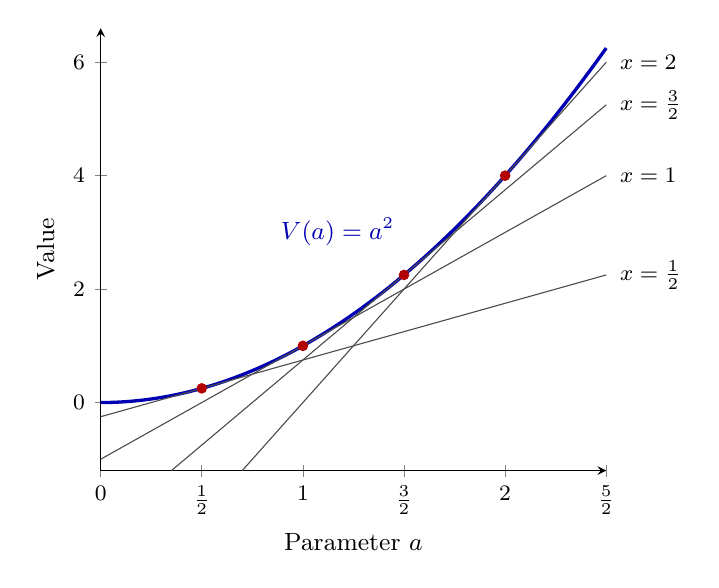
\begin{tikzpicture}
\begin{axis}[
  width=0.66\textwidth, height=7.2cm,
  xmin=0, xmax=2.5, ymin=-1.2, ymax=6.6,
  xlabel={Parameter $a$}, ylabel={Value},
  xtick={0,0.5,1,1.5,2,2.5}, xticklabels={$0$,$\frac{1}{2}$,$1$,$\frac{3}{2}$,$2$,$\frac{5}{2}$},
  tick label style={font=\footnotesize}, label style={font=\small},
  axis lines=left, clip=false]
  \addplot[domain=0:2.5, samples=100, very thick, blue!70!black] {x^2};
  \addplot[domain=0:2.5, samples=2, thin, black!70] {x - 0.25};
  \addplot[domain=0:2.5, samples=2, thin, black!70] {2*x - 1};
  \addplot[domain=0.35:2.5, samples=2, thin, black!70] {3*x - 2.25};
  \addplot[domain=0.7:2.5, samples=2, thin, black!70] {4*x - 4};
  \addplot[only marks, mark=*, mark size=1.7pt, red!70!black] coordinates {(0.5,0.25) (1,1) (1.5,2.25) (2,4)};
  \node[anchor=west, font=\footnotesize] at (axis cs:2.52,2.25) {$x = \frac{1}{2}$};
  \node[anchor=west, font=\footnotesize] at (axis cs:2.52,4) {$x = 1$};
  \node[anchor=west, font=\footnotesize] at (axis cs:2.52,5.25) {$x = \frac{3}{2}$};
  \node[anchor=west, font=\footnotesize] at (axis cs:2.52,6) {$x = 2$};
  \node[anchor=south east, font=\small, blue!70!black] at (axis cs:1.5,2.6) {$V(a) = a^2$};
\end{axis}
\end{tikzpicture}
\caption{The envelope theorem. Each thin line is $f(x, a) = 2xa - x^2$ for a fixed choice $x \in \{\frac{1}{2}, 1, \frac{3}{2}, 2\}$.
The value function $V(a) = \max_x f(x, a) = a^2$, attained at $x^*(a) = a$, is their upper envelope. Each line touches the
envelope at $a = x$ (dots), so $V'(a) = \frac{\partial f}{\partial a}(x^*(a), a) = 2x^*(a) = 2a$. The envelope is convex because
it is a maximum of functions linear in $a$.}
\label{fig:B-envelope}
\end{figure}

\subsection{The envelope theorem with constraints}\label{sec:B-envelope-constrained}

\begin{theorem}[Envelope theorem with constraints]\label{thm:B-envelope-constrained}
In problem \eqref{eq:B-constrained} with scalar $a$, let $f$ and the $g_k$ be $C^1$ in $(x, a)$. Suppose that near $a$
the solution $x^*(a)$ and multipliers $\lambda^*(a)$ are differentiable, satisfy the conditions of \cref{thm:B-kkt}, and
that the set of binding constraints does not change. Then
\begin{equation}\label{eq:B-envelope-constrained}
V'(a) = \frac{\partial \mathcal{L}}{\partial a}\big(x^*(a), \lambda^*(a), a\big)
= f_a\big(x^*(a), a\big) + \sum_{k}\lambda_k^*(a)\,\frac{\partial g_k}{\partial a}\big(x^*(a), a\big) .
\end{equation}
\end{theorem}

\begin{proof}
Write $V(a) = f(x^*(a), a)$ and differentiate:
\begin{equation*}
V'(a) = \nabla_x f^\top\frac{\dd x^*}{\dd a} + f_a .
\end{equation*}
Stationarity replaces $\nabla_x f$ by $-\sum_k\lambda_k^*\nabla_x g_k$:
\begin{equation*}
V'(a) = -\sum_k\lambda_k^*\,\nabla_x g_k^\top\frac{\dd x^*}{\dd a} + f_a .
\end{equation*}
A binding constraint satisfies $g_k(x^*(a), a) = 0$ on a neighborhood of $a$. Differentiating this identity gives
$\nabla_x g_k^\top\frac{\dd x^*}{\dd a} = -\frac{\partial g_k}{\partial a}$. A slack constraint has $\lambda_k^* = 0$ on a
neighborhood. Substituting both facts yields \eqref{eq:B-envelope-constrained}.
\end{proof}

\begin{corollary}[Multipliers as shadow prices]\label{cor:B-shadow}
If a constraint takes the form $h(x) \leq b$, the derivative of the value with respect to $b$ equals its multiplier,
$\frac{\partial V}{\partial b} = \lambda^*$.
\end{corollary}

\begin{proof}
Write the constraint as $g(x, b) = b - h(x) \geq 0$. Then $\frac{\partial g}{\partial b} = 1$, the objective does not depend
on $b$, and \eqref{eq:B-envelope-constrained} gives $V'(b) = \lambda^*$.
\end{proof}

In \cref{ex:B-cobb-douglas}, the budget constraint is $p^\top q \leq I$, and indeed $\frac{\partial v}{\partial I} = \frac{1}{I} = \lambda$.
The multiplier on a budget is the marginal utility of income, and the multiplier on an output constraint in cost
minimization is marginal cost (\cref{ex:B-shephard-cost}).

\begin{remark}[The Le Chatelier principle]\label{rem:B-lechatelier}
Split the choice into $x = (y, z)$, where $z$ is fixed at $\bar z$ in the short run. The long-run value
$V^L(a) = \max_{y, z}f(y, z, a)$ is at least the short-run value $V^S(a) = \max_yf(y, \bar z, a)$, with equality at the
$a_0$ for which $\bar z$ is optimal. The difference $V^L - V^S$ is therefore minimized at $a_0$. Its first derivative
vanishes there and its second derivative is nonnegative, so ${V^L}'(a_0) = {V^S}'(a_0)$ and
${V^L}''(a_0) \geq {V^S}''(a_0)$. When $V'$ is a supply or demand function, as with Hotelling's lemma below, long-run
responses are at least as large as short-run ones \citep{Samuelson1947}. For costs the inequality flips. Long-run cost
is the lower envelope of short-run cost curves and touches the one with the optimal capital stock. At that output,
long-run and short-run marginal cost coincide, and long-run marginal cost is flatter. This is one reason why
accounting measures of cost can differ from the economic marginal cost that pricing theory needs (\cref{ch:intro}).

Rationing gives a concrete case in consumer theory \citep[Section~4.3, pp.~110--112]{DeatonMuellbauer1980b}.
Let good 1 be rationed at the quantity the consumer would choose freely, $z = h_1(p, u)$, where $h$ is
Hicksian demand and $S_{jk} = \frac{\partial h_j}{\partial p_k}$ (\cref{sec:B-shephard}). Write
$h_j^*(p_{-1}, u, z)$ for the restricted Hicksian demand for good $j \neq 1$ (\cref{rem:B-rationing}). It does
not depend on $p_1$, and $h_j^*(p_{-1}, u, h_1(p, u)) = h_j(p, u)$ for all $p$ (their eq.~3.3).
\Cref{sec:05-welfare-virtual} differentiates this identity with respect to $p_1$ and $p_j$ and uses Slutsky
symmetry (\cref{prop:B-slutsky-matrix}). With $S_{11} < 0$, the restricted own-price effect is
\begin{equation*}
S^*_{jj} \equiv \frac{\partial h_j^*}{\partial p_j} = S_{jj} - \frac{S_{j1}^2}{S_{11}} \geq S_{jj},
\end{equation*}
their eq.~3.6 (p.~112). Both sides are nonpositive, so rationing good 1 weakly reduces the absolute
compensated own-price effect of every other good. The reduction is zero only when $S_{j1} = 0$.
\end{remark}

\subsection{Applications}\label{sec:B-envelope-apps}

\begin{example}[Hotelling's lemma]\label{ex:B-hotelling}
A price-taking firm with production function $\varphi(x)$, output price $p$ and input prices $r$ earns
\begin{equation*}
\pi(p, r) = \max_x\ p\,\varphi(x) - r^\top x .
\end{equation*}
\Cref{thm:B-envelope} gives
\begin{equation*}
\frac{\partial \pi}{\partial p} = \varphi(x^*) = q^* , \qquad \frac{\partial \pi}{\partial r_\ell} = -x_\ell^* ,
\end{equation*}
so supply and input demands are derivatives of the profit function \citep{Hotelling1932}. For each $x$, the objective is
linear in $(p, r)$. By \cref{lem:B-minlinear}, $\pi$ is convex in $(p, r)$. Its second derivatives therefore give
$\frac{\partial q^*}{\partial p} = \frac{\partial^2 \pi}{\partial p^2} \geq 0$ and $\frac{\partial x_\ell^*}{\partial r_\ell} = -\frac{\partial^2 \pi}{\partial r_\ell^2} \leq 0$:
supply curves slope up and input demand curves slope down.
\end{example}

\begin{example}[Shephard's lemma and marginal cost]\label{ex:B-shephard-cost}
The cost function is $C(r, q) = \min_x\{r^\top x : \varphi(x) \geq q\}$. Write it as the maximization problem
$-C(r, q) = \max_x\{-r^\top x : \varphi(x) - q \geq 0\}$, with Lagrangian $-r^\top x + \lambda(\varphi(x) - q)$.
\Cref{thm:B-envelope-constrained} gives
\begin{equation*}
\frac{\partial C}{\partial r_\ell} = x_\ell(r, q) , \qquad \frac{\partial C}{\partial q} = \lambda^* ,
\end{equation*}
the first being Shephard's lemma for costs \citep{Shephard1953}. The multiplier on the output constraint is marginal
cost. Stationarity reads $r_\ell = \lambda^*\frac{\partial \varphi}{\partial x_\ell}$, so each input price equals marginal cost times
the input's marginal product. Multiplying by $\frac{x_\ell}{q}$ for a freely adjustable input $\ell$ and dividing the output
price $p$ by $\lambda^*$,
\begin{equation*}
\frac{p}{\lambda^*} = \Big(\frac{\partial \varphi}{\partial x_\ell}\frac{x_\ell}{q}\Big)\frac{pq}{r_\ell x_\ell} .
\end{equation*}
The markup ratio equals the output elasticity of the flexible input times the ratio of revenue to spending on that
input. This is the production approach to markups (\cref{prop:01-production-markup}, \citealp{DeLoeckerWarzynski2012}).
Concavity of $C$ in $r$ follows from \cref{lem:B-minlinear}.
\end{example}

\begin{example}[Monopoly profit, cost and taxes]\label{ex:B-monopoly-tax}
A monopolist with constant marginal cost $c$ and specific tax $t$ earns $\pi^*(t) = \max_p(p - c - t)Q(p)$. The envelope
theorem gives $\frac{\dd \pi^*}{\dd t} = -Q(p^*)$. To first order, profit falls by the quantity sold whatever the
pass-through rate. Consumer surplus $\int_{p^*}^{\infty}Q(u)\,\dd u$ falls at rate $Q\frac{\dd p^*}{\dd t} = \rho Q$ by Leibniz's
rule. The ratio of consumer to producer burden under monopoly is therefore $\rho$, the case $\theta = 1$ of
\cref{prop:02-incidence}.
\end{example}

\begin{example}[Entry lowers incumbents' Cournot profits]\label{ex:B-cournot-entry}
Firm $i$'s profit given rivals' output is $V_i(Q_{-i}) = \max_{q_i}\big[P(q_i + Q_{-i})q_i - C_i(q_i)\big]$. By the envelope
theorem,
\begin{equation*}
V_i'(Q_{-i}) = q_i\,P'(Q) < 0 \qquad\text{whenever } q_i > 0 .
\end{equation*}
The firm's own output response has no first-order effect. In a symmetric equilibrium with $N$ firms, rivals' output is
$Q_{-i} = Q - q$, and entry raises it, since $\frac{\dd Q}{\dd N} > 0$ and $\frac{\dd q}{\dd N} < 0$ (\cref{prop:02-entry-cs}).
Treating $N$ as continuous,
\begin{equation*}
\frac{\dd \pi}{\dd N} = q\,P'(Q)\Big(\frac{\dd Q}{\dd N} - \frac{\dd q}{\dd N}\Big) < 0 .
\end{equation*}
\end{example}

\begin{example}[Bidder rents in the first-price auction]\label{ex:B-auction-envelope}
There are $n$ bidders with independent private values drawn from $F$, and a reserve price $r$. Rivals use a strictly
increasing bid function $\beta$ with $\beta(r) = r$. A bidder with value $v \geq r$ who bids $\beta(z)$ wins when every rival
value is below $z$, with probability $F(z)^{n - 1}$. Her equilibrium payoff is
\begin{equation*}
\pi(v) = \max_{z}\ \big(v - \beta(z)\big)F(z)^{n - 1} ,
\end{equation*}
and in equilibrium $z = v$ is optimal. For each $z$ the objective is affine in $v$ with slope $F(z)^{n - 1}$. So $\pi$ is a
maximum of affine functions, hence convex and absolutely continuous, and \cref{thm:B-envelope-integral} applies:
\begin{equation*}
\pi'(v) = F(v)^{n - 1} \ \text{almost everywhere}, \qquad \pi(r) = \big(r - \beta(r)\big)F(r)^{n - 1} = 0 .
\end{equation*}
Integrating from $r$ gives $\pi(v) = \int_r^vF(t)^{n - 1}\,\dd t$. The payoff is also the winning probability times the
surplus when winning, $\pi(v) = (v - \beta(v))F(v)^{n - 1}$. Equating the two expressions,
\begin{equation*}
\beta(v) = v - \frac{\int_r^vF(t)^{n - 1}\,\dd t}{F(v)^{n - 1}} ,
\end{equation*}
which is \eqref{eq:B-rs-bid}. With uniform values on $[0, 1]$ and $r = 0$, $\beta(v) = \frac{n - 1}{n}v$.

The first-order route reaches the same formula with more work. Differentiating the objective in $z$ at $z = v$ gives
$-\beta'(v)F(v)^{n - 1} + (v - \beta(v))(n - 1)F(v)^{n - 2}f(v) = 0$. Rearranged, this is the differential equation
\begin{equation*}
\frac{\dd}{\dd v}\Big[\beta(v)F(v)^{n - 1}\Big] = v\,\frac{\dd}{\dd v}\Big[F(v)^{n - 1}\Big] .
\end{equation*}
Integrating from $r$ and applying the integration by parts of \cref{ex:B-rs-parts} gives the bid again. The envelope
route needs neither the differential equation nor differentiability of $\beta$. It also shows that the payoff
$\pi(v)$ depends only on who wins and on the zero payoff of type $r$. Any format with the same allocation and
$\pi(r) = 0$ therefore yields the same expected payments, which is revenue equivalence \citep{Myerson1981,
RileySamuelson1981}. \Cref{sec:14-fpa-envelope} develops these results.
\end{example}

\begin{example}[Expected maximum utility]\label{ex:B-logsum-envelope}
Let $\mathcal{W}(\delta) = \E[\max_k(\delta_k + \epsilon_k)]$ in an additive random utility model with continuously distributed
errors. For each realization of $\epsilon$, the maximum is the value of a choice over a finite set. Its derivative in
$\delta_j$ is $\indic\{j \text{ is the maximizer}\}$ wherever the maximizer is unique, which holds with probability one.
This is the envelope theorem for a finite choice set. Taking expectations,
\begin{equation*}
\frac{\partial \mathcal{W}}{\partial \delta_j} = \Pr(j \text{ is chosen}) = s_j(\delta) .
\end{equation*}
The exchange of derivative and expectation needs a domination argument, which the Williams-Daly-Zachary theorem
(\cref{thm:B-wdz}) supplies. In the logit, $\mathcal{W} = \ln\sum_ke^{\delta_k}$ plus a constant, and
$\frac{\partial}{\partial \delta_j}\ln\sum_ke^{\delta_k} = s_j$.
\end{example}
